\chapter{Resource Dimensioning and Management Schemes in Clouds}\label{chap:cloud}

In this chapter we consider stakeholder tradeoffs in cloud scenarios.
Traditionally, a cloud is a set of compute and network resources, which can be elastically rented by customers.
The recent rise of crowdsourcing platforms, also described as human-cloud, it has become useful to refer to this type of cloud as \emph{machine cloud}, in order to better differentiate these two types of cloud.
The human-cloud is based on the sample principles as the machine cloud, e.g. elasticity and reliability and enabled crowdsourcing employers to offer tasks to workers available on demand.
In this chapter we consider multiple scenarios:
First, we study the role of a cloud operator providing virtual resources to customers.
Then, we consider decisions faced by a user of a cloud who is deploying virtualised network functions in a cloud.
Finally, we investigate resource dimensioning in human-clouds.
Regardless of the specific scenario, the number of resources available impact the \glspl{KPI} of all participating stakeholders, and is thus subject to optimisation.

\begin{figure}
  \centering
  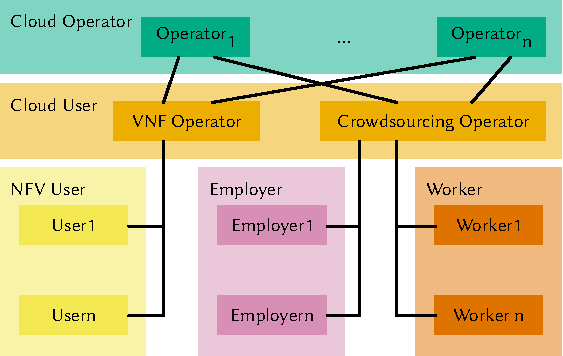
\includegraphics{cloud/figures/model}
  \caption{Stakeholders investigated in the cloud scenarios.}
  \label{fig:cloud:model}
\end{figure}

We first provide an overview of the involved stakeholders and \glspl{KPI} in \reffig{fig:cloud:model}.
If we study the operation of a machine cloud, both the cloud operator and the cloud user need to be considered.
The cloud operator is interested in increasing revenue, i.e. attracting a high number of customers, and decrease financial expenditure, e.g. by reducing consumed energy.
The customer of a cloud operator is interested in good \glspl{SLA}, for example a low delay before processing of a job can begin.
In the second scenario, the network function operator taking the role of a customer in the previous scenario, is interested in provisioning a minimal number of resources from the cloud operator, in order to reduce cost, while in turn providing a sufficient \gls{SLA} to its customers.
The users of the virtualised network functions demand a sufficient availability of the provided service.
Finally, in case of the human-cloud scenario, the cloud operator has to satisfy two stakeholders with conflicting interests.
On the one hand, employers are interested in a fast completion of the offered tasks.
On the other hand, workers are interested in obtaining a high income.
These goals are clearly conflicting, as fast completion can be obtained by providing a high number of available workers.
However, income per workers increases if the tasks are distributed between fewer workers.
Thus, the human-cloud operator has to balance the interests of the two stakeholders.

The contribution of this chapter is threefold
\begin{enumerate}
\item We provide a model for energy-efficient data centre operation and discuss sensible parameter configurations for the different stakeholders. 
\item We study algorithms for resource provisioning on the example of a virtualised network function and evaluate their performance with respect to the demands of the stakeholders.
\item We model a crowdsourcing platform and provide guidelines for platform operators regarding resource acquisition.
\end{enumerate}

The content of this chapter is published in~\cite{Schwartz2012a,Metzger2014a,Schwartz2015}.
In \refsec{sec:cloud:related_work} we provide an overview of related work relevant to this chapter.
Then, in \refsec{sec:cloud:data_centers} we discuss the tradeoffs faced by a cloud operator.
We focus on the customer of a cloud operator in \refsec{sec:cloud:virtualized_network_functions} and discuss challenges when provisioning virtualised network functions.
Strategies for resource provisioning of a human-cloud are considered in \refsec{sec:cloud:crowdsourcing}.
Finally, we provide lessons learned from our studies in \refsec{sec:cloud:lessons_learned}.

\section{Background and Related Work}\label{sec:network:background}
This section discusses the technical background relevant to the remainder of this chapter.
First, in \refsec{sec:network:background:umts_rrc} we introduce the \gls{UMTS} mobile communication standard, and the \gls{RRC} protocol.
Then we discuss existing aproaches to measure \gls{RRC} protocol transactions and optimise the signalling load generated by \gls{RRC} messages in \refsec{sec:network:background:measurement_optimisation}.
Finally, \refsec{sec:network:background:energy_consumption_qoe} tackles smartphone power consumption and \gls{QoE}, two metrics influenced by the configuration of the \gls{RRC} protocol.

\subsection{\headershortacr{UMTS} Networks and the \headershortacr{RRC} Protocol}\label{sec:network:background:umts_rrc}
A \gls{3G} \gls{UMTS} mobile network consists of three main components, which are depicted in \reffig{fig:network:background:mobile_network_overview}: The \gls{UE}, the \gls{RAN}, and the \gls{CN}.
The \gls{RAN} is used to establish connectivity between the \gls{UE} and the \gls{CN}, which in turn can establish connectivity to the Internet, if required.

\begin{figure}
	\centering
	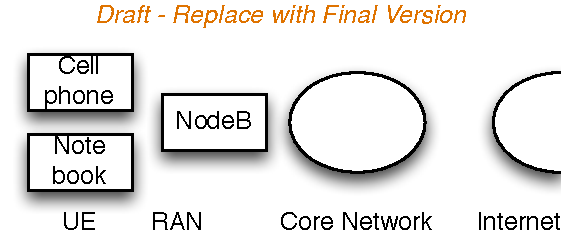
\includegraphics{network/background/figures/mobile_network_overview}
	\caption{Overview of Mobile Network}
	\label{fig:network:background:mobile_network_overview}
\end{figure}

\gls{UE} consists of devices used by end users, i.e. smartphones, tablets or data card enabled notebooks, but can also include \gls{M2M} devices.
The \gls{RAN} is, amongst other tasks, responsible for \gls{RRC}, packet scheduling and handover control.
It includes network entities such as the \gls{NodeB} and the \gls{RNC}.
The \gls{CN} provides the backbone network of the \gls{UMTS} network and provides connectivity to the Internet and the \gls{PSTN}.
Furthermore, functionality such as billing, authentication and location management is provided by the \gls{CN}.

In UMTS networks, the radio resources in the RAN between base station and UE are controlled and managed by the \gls{RRC} protocol~\cite{3GPP_RRC_Spec}.
The protocol offers services such as broadcast of network information, maintenance of a connection between the \gls{UE} and \gls{RAN}, establishment of point-to-point radio bearers for data transmission, \gls{QoS} control, and reporting and cell selection management.
The protocol is divided into different parts: services for upper layers, communication with lower layers, protocol states, \gls{RRC} procedures, and error control.
In particular, \gls{RRC} also participates in the co-ordination of other resource management operations such as channel measurements and handovers.
All \gls{RRC} procedures rely on protocol states which are defined to trigger action should be applied and which information must be signaled. 
The state are defined per \gls{UE} and for the connection between the \gls{UE} and the \gls{NodeB} station.
Typically there are five \gls{RRC} states characterizing a connection between \gls{UE} and \gls{NodeB}: \texttt{idle}, \texttt{URA\_PCH}, \texttt{CELL\_PCH}, \texttt{RRC\_DCH}, and \texttt{RRC\_FACH}.
Whether a specific \gls{RRC} state is used in a specific mobile network depends on the configuration of the network by the provider.
In the following we concentrate on the most commonly observed~\cite{Qian2010a} \gls{RRC} states \gls{RRC_idle}, \gls{RRC_DCH}, and \gls{RRC_FACH}.
We neglect \texttt{URA\_PCH} and \texttt{CELL\_PCH} in this study.
While \texttt{URA\_PCH} plays only a role in scenarios of high mobility, \texttt{CELL\_PCH} is not yet widely implemented. 
Our results are still of general nature and do not depend on the limited number of considered \gls{RRC} states.

If the \gls{UE} is switched on and no connection to the mobile network is established, the \gls{UE} is in \gls{RRC_idle} state.
If the \gls{UE} wants to send data, radio resources are allocated by the \gls{NodeB} for the handset and the \gls{UE} will transition to either the \gls{RRC_FACH} or the \gls{RRC_DCH} state. 
Then, a corresponding channel for data transmission is assigned to the \gls{UE}.
The \gls{RRC_FACH} and the \gls{RRC_DCH} state can be distinguished in that way that in \gls{RRC_DCH} state a high-power dedicated channel for high speed transmission is allocated whereas in \gls{RRC_FACH} state a shared access channel for general sporadic data transmission is used.
Thus, \gls{RRC_FACH} consumes significantly less power than the \gls{RRC_DCH} state. 

The possible transitions between the different states are defined by the network operator and the \gls{RRC} protocol stack.
Typically, the following state transitions are included: 
\gls{RRC_idle} \(\rightarrow\) \gls{RRC_FACH},
\gls{RRC_FACH} \(\rightarrow\) \gls{RRC_DCH} to switch from lower radio resource utilization and low \gls{UE} energy consumption to another state using more resources and energy, and 
\gls{RRC_DCH} \(\rightarrow\) \gls{RRC_FACH}, 
\gls{RRC_FACH} \(\rightarrow\) \gls{RRC_idle},
\gls{RRC_DCH} \(\rightarrow\) \gls{RRC_idle} to switch to lower resource usage and energy consumption.
According to~\cite{Perala2009,Qian2010a}, the transitions are triggered by user activity and radio link control buffer level. 
A transition from \gls{RRC_DCH} to \gls{RRC_FACH} usually occurs when the buffer is empty and a threshold for a release timer is exceeded, resulting into the corresponding \gls{RRC} protocol message flow.
A transition in the reverse direction is triggered if the buffer level exceeds a specified threshold value for a predefined time period.
The \gls{UE} will transition into \gls{RRC_idle} state if the \gls{RNC} detects overload in the network or no data was sent by the \gls{UE} for a specified time.

\begin{figure}
	\begin{subfigure}[b]{.5\textwidth}
	\centering
	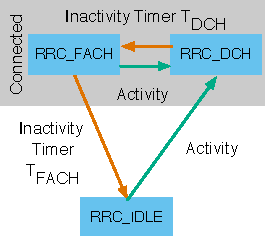
\includegraphics{network/background/figures/three_states}
	\caption{Three State Scenario}\label{fig:network:background:rrc_state_machines:three_states}
	\end{subfigure}
	\begin{subfigure}[b]{.5\textwidth}
	\centering
	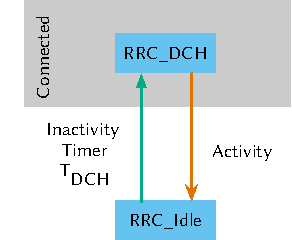
\includegraphics{network/background/figures/two_states}
	\caption{Two State Scenario}\label{fig:network:background:rrc_state_machines:two_states}
	\end{subfigure}
	\caption{\headershortacr{RRC} State Machine Diagrams}\label{fig:network:background:rrc_state_machines}
\end{figure}

In the following, we consider two different state transition models, depicted in \reffig{fig:network:background:rrc_state_machines}, based on the \gls{RRC} protocol.
The first model includes the \gls{RRC_idle}, \gls{RRC_FACH}, and \gls{RRC_DCH} states is shown in \reffig{fig:network:background:rrc_state_machines:three_states} and is in the following called the three state model.
If the \gls{UE} is in the \gls{RRC_idle} state and activity is detected, i.e. a packet is sent or received, the connection transitions to \gls{RRC_DCH} state.
After each transmission a timer \gls{TDCH} is started and reset whenever a new packet is sent or received.
If the timer expires, the connection transitions to the \gls{RRC_FACH} state
Upon entering, the \gls{TFACH} timer is started.
If a new transmission occurs, the connection again transitions to the \gls{RRC_DCH} state.
If \gls{TFACH} expires, the connection transitions to \gls{RRC_idle} state.

The second model, denoted as the two state model, and shown in \reffig{fig:network:background:rrc_state_machines:two_states}, only includes the \gls{RRC_idle} and \gls{RRC_DCH} state.
If the \gls{UE} is in the \gls{RRC_idle} mode and a packet is sent or received, the connection transitions to the \gls{RRC_DCH} state. Once in \gls{RRC_DCH} mode, the \gls{TDCH} timer is started and it is reset whenever a new packet is sent or received.
If the timer expires, the \gls{UE} transitions back to \gls{RRC_idle} state.

While the three state model is closer to the specified \gls{RRC} protocol is similar to some proprietary \emph{Fast Dormancy} implementations used by \gls{UE} vendors.
In these Fast Dormancy implementations, the \gls{UE} tears down the connection to the network state as soon as no data is ready to be sent for a certain time, i.e., it forces the network to transition to \gls{RRC_idle} state.
In contrast to the three state model, there is no transition to the \gls{RRC_FACH} state.
If a device disconnects from the network by transitioning to the \gls{RRC_idle} state, it has to be reauthenticated before another transition to the \gls{RRC_DCH} state can occur.
This results in additional signalling traffic and causes more load on the network \cite{NSN2011} due to frequent re-establishments of the RRC connection.
These proprietary Fast Dormancy algorithms do not adhere to the \gls{RRC} specification \cite{GSM2010}, but nontheless exist in the real world and have been identified as possible causes for signalling storms.
The major reason for Fast Dormancy implementations is the decrease in power consumption on the \gls{UE}, since the transmission unit of the \gls{UE} consumes only \SIrange{1}{2}{\percent} of the energy in \gls{RRC_idle} state compared to the \gls{RRC_DCH} state.
Thus, both models warrant further investigation.

\subsection{Measurements of \headershortacr{RRC} Parameters and Optimisation of Resource Consumption}\label{sec:network:background:measurement_optimisation}

In the literature, the configuration of the inactivity timers used for the \gls{RRC} protocols have been investigated in detail.
In~\cite{Perala2009} a measurement tool for \gls{RRC} protocol states is presented. 
It is used to determine \gls{RRC} state transition parameters, channel setup delays, and paging delay by measuring the one-way round trip time of data packets.
The results are validated by monitoring the energy consumption in different \gls{RRC} states.
One outcome is that \gls{UMTS} network configurations vary significantly by network operator.
\gls{RRC_DCH} release timer as well as the inactivity timer value triggering transition to \gls{RRC_idle} state were measured.
The values range from \SI{1.2}{\second} for the \gls{RRC_DCH} release timer to more than one minute for the \gls{RRC_idle} timer.
Similar results are presented in~\cite{Qian2010a}.
Here, the observed values vary between \SI{5}{\second} and \SI{12}{\second}. 
Additionally, they also determined the exact \gls{RRC} state transitions for two networks such as \gls{RRC_idle} \(\rightarrow\) \gls{RRC_FACH} \(\rightarrow\) \gls{RRC_DCH} or \gls{RRC_idle} \(\rightarrow\) \gls{RRC_DCH} directly without transitioning through the \gls{RRC_FACH} state.
The \gls{3GPP} has released a technical report \cite{3GPP_22801} about the adverse impact of mobile data applications.
This report states that frequent connection re-establishments due to small data packets caused e.g. by status updates of social network or instant messaging apps can lead to problems of increased signalling load.
This highlights the importance of this topic.

Furthermore, there are papers that propose optimizing strategies that take the \gls{RRC} states into account. 
In~\cite{Qian2011} the impact of different application traffic patterns is studied to reveal resource usage in mobile networks.
By identifying packet bursts, they infer the \gls{RRC} states of the \gls{UE}.
Radio resources are quantified by channel occupation time and energy consumption.
They propose an algorithm that tries to optimize application traffic patterns by e.g. piggybacking, batching up data, or decreasing the update rate of an application.
The algorithm is evaluated for six applications, two news applications, Pandora streaming application, Google search, Tune-In radio and Mobelix. 
In~\cite{Qian2010b} also \gls{RRC} states are studied for network optimization.
The authors optimize the inactivity timers to allow a better resource utilization. 
They propose a application-to-network interface to avoid unnecessary timer periods after data transmission.

\subsection{Smartphone Power Consumption and \headershortacr{QoE}}\label{sec:network:background:energy_consumption_qoe}
Power consumption of the \gls{UE} varies according to the devices current \gls{RRC} state.
The power consumption caused by \gls{RRC_DCH} mode was measured at about \SIrange{600}{800}{\milli\watt}~\cite{Qian2011,Qian2010a}.
In \gls{RRC_FACH} mode, the consumption was measured at about \SIrange{400}{460}{\milli\watt} depending on the \gls{UE} and the network operator~\cite{Qian2010a}.
A precise measurement of the power consumption of different \gls{RRC} states is performed in~\cite{Qian2010a,Balasubramanian2009,Lee2004}. 
The authors report that the energy drain depends on two factors: 
\begin{enumerate*}
\item user interactions and applications 
\item platform hardware and software.
\end{enumerate*}

In \cite{Ickin2012} the authors performed a 4 week long study with 29 participants to identify factors influencing \gls{QoE} of mobile applications.
The study comprises
\begin{enumerate*}
\item data from context sensing software,
\item user feedback using an experience sampling method several times per day, and
\item weekly interviews of the participants.
\end{enumerate*}
To determine the factors of influence, the authors analyze the frequency of specific keywords in the interviews and the surveys.
They find that the term \emph{battery} has the highest frequency.
According to the authors this is reasonable since the battery efficiency has a strong impact on the user perceived quality, in particular when it the \gls{UE} is nearly discharged.
\section{Data Centres}\label{sec:cloud:data_centers}
Data centres are used to host most of the applications running in the Internet, including those discussed earlier in this work.
Servers are operated by the data centre operator and rented out to customers as part of a \gls{PaaS} or \gls{IaaS} scheme.
In order to increase revenue the data centre operator is interested in decreasing server power drain, one of the major matters of expense for data centres \cite{Greenberg2009b}, while satisfying \glspl{SLA} with their customers.

This section studies this scenario and provides a model intended for data centre operators to manage this tradeoff.
In \refsec{sec:cloud:data_centers:problem_formulation} we provide a mathematical formulation for the considered scenario.
Then, in \refsec{sec:cloud:data_centers:modeling} we model this scenario using methods from queueing theory and derive metrics which can be used to evaluate the different approaches and configurations of data centres.
In \refsec{sec:cloud:data_centers:closed_form_solution} we present different methods for solving the previously introduced queueing model.
Finally, in \refsec{sec:cloud:data_centers:performance_evaluation} we study the performance implications of the model and discuss the tradeoff between power drain and suffered waiting time.

\subsection{Problem Formulation}\label{sec:cloud:data_centers:problem_formulation}

A widely used data center architecture is the three-tier architecture shown in \reffig{fig:sec:cloud:data_centers:problem_formulation:3-tier_datacenter}.
The upper two layers of the architecture are responsible for distributing the traffic and consist of layer 3 switches where each switch has a backup switch.
In this paper, we focus on the edge layer and here on a single \gls{POD}.
A \gls{POD} consists of a number of servers connected over top of rack switches to an aggregation switch.

\begin{figure}
  \centering
  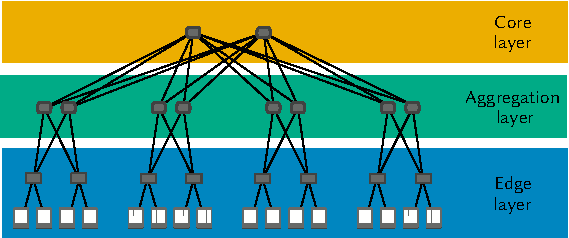
\includegraphics{cloud/data_centers/problem_formulation/figures/architecture}
  \caption{Three-tier data center architecture}
  \label{fig:sec:cloud:data_centers:problem_formulation:3-tier_datacenter}
\end{figure}


We assume, that new jobs entering the system arrive with exponentially distributed inter-arrival time.
When a job in form of a packet arrives at the \gls{POD}, it is forwarded to an idle server.
If no idle server is available, the job is queued.
Once a server finishes processing its current job, it picks another one from the queue.

Our goal is now to evaluate how much power is consumed in a data center and how much can be saved when servers, not processing any job, are switched off.
Therefore, we developed two different data center models.
The first model, the \emph{default data center}, consists of two-state servers only which are either \emph{busy} or \emph{idle}, as shown in \reffig{fig:sec:cloud:data_centers:problem_formulation:servers:idle_busy}) 
For the second model, a more \emph{energy-efficient data center}, a subset of the servers may additionally be switched on and \emph{off} on demand, shown in \reffig{fig:sec:cloud:data_centers:problem_formulation:servers:idle_busy_off} as recommended in~\cite{EPA2007}.

\begin{figure}
	\begin{subfigure}[b]{\textwidth}
	\centering
	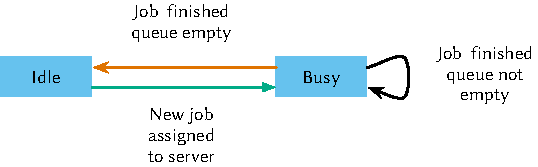
\includegraphics{cloud/data_centers/problem_formulation/figures/idle_busy}
	\caption{2-state server model}\label{fig:sec:cloud:data_centers:problem_formulation:servers:idle_busy}
	\end{subfigure} 
	\begin{subfigure}[b]{\textwidth}
	\centering
	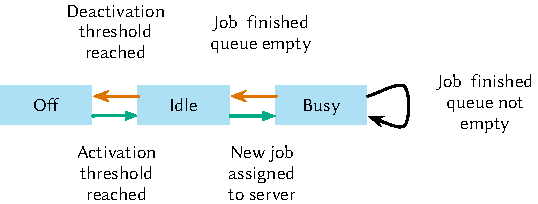
\includegraphics{cloud/data_centers/problem_formulation/figures/idle_busy_off}
	\caption{3-state model of a reserved server}\label{fig:sec:cloud:data_centers:problem_formulation:idle_busy_off}
	\end{subfigure}

	\caption{CPower state transition on a per server level}\label{fig:sec:cloud:data_centers:problem_formulation:servers}
\end{figure}

\subsection{Default Data Center}\label{sec:cloud:data_centers:problem_formulation:default_data_center}
For the default data center model, each of the \(n\) servers is either on and processing a job or on and idle as depicted in \reffig{fig:sec:cloud:data_centers:problem_formulation:servers:idle_busy}.
If a busy server finishes processing a job and the queue is empty, the server becomes idle. Once a new job is assigned to a yet idle server, the server becomes busy.
According to our measurements of a server with an Intel twelve core processor \SI{2.67}{\giga\hertz} and \SI{32}{\giga\byte} RAM, a server currently processing a job consumes \(e_{\text{busy}} = \SI{240}{\watt}\)
An idle server still consumes \(e_{\text{idle}} = \SI{170}{\watt}\).

\subsection{Energy-Efficient Data Center}\label{sec:probform_3states}
For the second model, we differentiate between two types of servers.
\(n\) base-line servers which are always on and \(m\) reserved servers to be enabled on demand.
If they are enabled, their power consumption is similar to that of the default data center model.
If they are disabled, each server consumes \(e_\text{off} = \SI{0}{\watt}\).
The \(n\) servers which are always enabled consume the same power as in the default data center model.
If the system queue has a length exceeding \(\theta_2\) where \(\theta_2 \in (0, m)\) holds, the \(m\) reserved servers are enabled and stay enabled until the total number of jobs in the system drops to \(\theta_1\) for \(\theta_1 \in (0, n)\).
The transition between power levels for each of the reserved servers is depicted in \reffig{fig:sec:cloud:data_centers:problem_formulation:idle_busy_off}.

The energy-efficient data center operation model with the parameters \(\theta_1\) and \(\theta_2\) is depicted in \reffig{fig:sec:cloud:data_centers:problem_formulation:model} and described in detail in the next section.

\begin{figure}
  \centering
  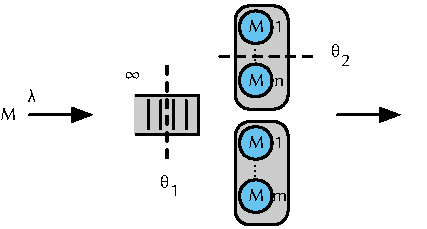
\includegraphics{cloud/data_centers/problem_formulation/figures/model}
  \caption{System model for an energy-efficient operation}
  \label{fig:sec:cloud:data_centers:problem_formulation:model}
\end{figure}
\subsection{Modeling}\label{sec:cloud:data_centers:modeling}
In this section, we first discuss the default data center model, where a server can either be idle or busy, processing a job. Afterwards, the energy-efficient data center model with the three states is set up.

\subsubsection*{Default Data Center}\label{sec:cloud:data_centers:modeling:default}
We consider new jobs arriving at a \gls{POD} with exponential \gls{IID} inter-arrival times with rate \(\lambda\) and each server accepts only one job at a time with an exponentially distributed service time with mean \(\frac{1}{\mu}\).
Then, the system can be modeled using a simple \(M/M/n\) delay system.
Here, the random variable \(X\) gives the number of jobs in the system and \(x(i)\) is the stationary probability that \(i\) jobs are currently in the system.

\subsubsection*{Energy Efficient Data Center}\label{sec:cloud:data_centers:modeling:energy_efficient}
\subsection{Analysis of Proposed Data Centre Models}\label{sec:cloud:data_centers:closed_form_solution}
Using the macro state equations discussed in \refsec{sec:cloud:data_centers:modeling}, there are multiple ways to obtain the state probabilities.
This section examines the different approaches.

\subsubsection*{System of Linear Equations}
First, it is possible to directly solve the system of linear equations implied by the micro or macro states.
Solvers for linear equation systems scale cubic in the dimension of the matrix, which in this case is bounded by the system size.
Especially for a large numbers of server, this prevents an exhaustive search of the parameter space.

\subsubsection*{Closed-form Solutions}
Thus, we obtain closed form solutions for the state probabilities.
These equations can be derived by recursively applying the macro state equations.

All equations feature a factor \(x(0, 0)\) which in turn can be calculated using the normalisation property given in \refeq{eq:cloud:data_centers:modeling:normative}.
Due to the length of the individual formulas, the following shorthand is introduced:
For each state probability \(x(i, j)\) depending on the factor \(x(0,0)\) we define \(\bar{x}(i, j) = x(i, j) \cdot x(0, 0)^{-1}\), i.e. we cancel the factor.

For \(0 < i <\theta_1\), we get
\begin{align*}
x(i, 0) &= x(0, 0) \cdot \frac{a^i}{i!}.
\end{align*}
As a further shorthand for substitution, we define
\begin{align*}
s_i&=\sum_{k=0}^{i}a^k(n-k-1)!.
\end{align*}
Using this definition, we get the state probability for \(\theta_1\) jobs in the system with activated reserved servers as
\begin{align*}
x(\theta_1, 1) &= x(0, 0)\cdot \frac{a^{n+\theta_2+1}}{\left(1+\frac{a}{\theta_1}\right)}
\cdot\frac{\left(\theta_1-1\right)!\left(\frac{(1-a^{\theta_2})\theta_1}{1-a}+a^{\theta_2}s_{n-\theta_1}\right)}{n^{\theta_2}n!\left(n-\theta_1+1\right)!}.
\end{align*}
For \(\theta_1\leq i\leq n\), we get
\begin{align*}
x(i, 0) = x(0, 0) &\cdot \left(\frac{\bar{x}(n, 0) a^{i-\theta_1+1}}{(i-\theta_1+1)!} - \frac{\bar{x}(\theta_1,1) \theta_1 s_{i-\theta_1}}{i!}\right).
\end{align*}
And for \(n<i\leq n+\theta_2\), we get
%TODO single line
\begin{align*}
x(i, 0) = x(0, 0) &\cdot \left(\frac{\bar{x}(n,0) a^{i-\theta_1+1}}{n^{i-n}(n-\theta_1+1)!}\right.\\
&\left.-\bar{x}(\theta_1,1)\left(\frac{\theta_1 s_{n-\theta_1} a^{i-n}}{n!} + \frac{\theta_1(1-a^{i-n})}{1-a}\right)\right).
\end{align*}

Thus, we have all probabilities for system states where only the baseline servers are active. For the reserved servers, we obtain state probabilities for \(\theta_1<i\leq n+\theta_2+1\) as
\begin{align*}
x(i, 1) = x(0, 0) \cdot \left(\bar{x}(\theta_1, 1)\frac{a^{i-\theta_1}\theta_1!}{i!} + \bar{x}(n+\theta_2,0)\sum_{k=1}^{i-\theta_1}\frac{a^k(i-k)!}{i!}\right).
\end{align*}

For \(n+\theta_2+1 < i \leq n + m\), we get
\begin{align*}
x(i, 1) = x(0, 0)\cdot \bar{x}(n+\theta_2+1,1) \cdot\frac{a^{i-(n+\theta_2+1)}(n+\theta_2+1)!}{i!},
\end{align*}
and finally for \(i>n+m\)
\begin{align*}
x(i, 1) = x(0, 0)\cdot \bar{x}(n+m,1) \left(\frac{a}{n+m}\right)^{i-(n+m)}.
\end{align*}
As discussed earlier, the probability of an empty system is given by the normalisation condition:
\begin{align*}
x(0, 0)=\left(1 +\sum_{k=1}^{n+\theta_2}\bar{x}(k, 0) + \sum_{k=\theta_1}^{\infty}\bar{x}(k,1)\right)^{-1}.
\end{align*}

While these closed form solutions allow for the derivation of analytical properties of the model, performing a numerical analysis of a given parameter space is difficult due to numerical instability of the equations.

\subsubsection*{Recursive Algorithm}
To avoid these problems, we introduce a recursive algorithm to calculate the state probabilities based on the macro state equations.
To this end, our we first define \(x(0,0)\) as a constant \(K_0\), and then iteratively computes the state probabilities.
For an earlier application of this concept, see \cite{Trangia1997}.
First, we calculate \(x(i,0)\) for \(0<i<\theta_1\) as a factor of \(x(0,0)\) using \refeq{eq:cloud:data_centers:modeling:energy_efficient:S1_1}.
To obtain the probability for \(x(\theta_1,0)\), not only \(x(\theta_1 -1, 0)\), but \(x(\theta_1, 1)\) is required, which we have not obtained yet.
As this is the case with all \(x(i,0)\) for \(\theta_1 \leq i \leq n + \theta_2\) we implicitly introduce a second constant \(K_1\) for \(x(\theta_1, 1)\) and calculate all \(x(i,0)\) for \(\theta_1 \leq i \leq n + \theta_2\) as a linear combination of \(x(\theta_1 - 1,0)\) and \(K_1\) as follows:
\begin{equation}
x(i, 0) = x(\theta_1 - 1, 0) u_i + K_1 v_i.\label{eq:cloud:data_centers:modeling:closed_form_solution:linear_combination}
\end{equation}
For \(i = \theta_1\), \refeq{eq:cloud:data_centers:modeling:energy_efficient:S1_2} requires \(u_{\theta_1} = \frac{a}{\theta_1}\) and \(v_{\theta_1} = 1\).
Continuing this pattern by successively applying \refeq{eq:cloud:data_centers:modeling:energy_efficient:S1_2} for \(\theta_1 < i \leq n\), we get
\begin{align*}
u_i &= \frac{a}{i}u_{i-1},\\
v_i &= \frac{a}{i}v_{i-1} + \frac{\theta_1}{i}.
\end{align*}
We use \refeq{eq:cloud:data_centers:modeling:energy_efficient:S1_3} to continue for \(n < i \leq n + \theta_2\), and get
\begin{align*}
u_i &= \frac{a}{n}u_{i-1},\\
v_i &= \frac{a}{n}v_{i-1} + \frac{\theta_1}{n}.
\end{align*}
Thus, we arrive at a probability for \(x(n + \theta_2,0)\) depending on \(x(\theta_1 -1,0)\), which we have obtained, and \(K_1 = x(\theta_1,1)\) which we still need to acquire:
\begin{equation*}
x(n+\theta_2,0) = x(\theta_1 -1,0) u_{n+\theta_2} - K_1 v_{n+\theta_2}.
\end{equation*}
We apply \refeq{eq:cloud:data_centers:modeling:energy_efficient:S3} and solve for \(K_1\) and obtain
\begin{equation*}
K_1 =  \frac{\frac{a}{\theta_1} u_{n+\theta_2}}{\frac{a}{\theta_1} v_{n + \theta_2} + \theta_1} x(\theta_1 - 1, 0),
\end{equation*}
which allows to calculate the probabilities of \(x(i,0)\) for \(\theta_1 \leq i \leq n + \theta_2\) using \refeq{eq:cloud:data_centers:modeling:closed_form_solution:linear_combination}.

We can now obtain the probabilities for states in which the reserved servers have been activated, beginning with \((\theta_1 + 1,1)\) we apply \refeq{eq:cloud:data_centers:modeling:energy_efficient:S2_1} for all \(\theta_1 < i \leq n + \theta_2 + 1\) and get
\begin{equation*}
x(i,1) = \frac{a}{i}(x(i-1,1)+ x(n+\theta_2,0))
\end{equation*}
which we can calculate directly as all probabilities are known in relation to \(K_0\).
We continue applying \refeq{eq:cloud:data_centers:modeling:energy_efficient:S2_2} and obtain
\begin{equation}
x(i,1) = \frac{a}{i}(x(i-1,1) + x(n+\theta_2,0))\label{eq:cloud:data_centers:modeling:energy_efficient:probability_greater_nm}
\end{equation}
for \(n + \theta_2 + 1 < i \leq n + m\).

Finally, we need to calculate the probability that the system is in states \((i,1)\) for \(i > n + m\) where we need to obtain
\begin{equation*}
x(i>n+m,1) = \sum_{i = n + m + 1}^{+ \infty} x(i,1).
\end{equation*}
Due to the recursive definition of \refeq{eq:cloud:data_centers:modeling:energy_efficient:S2_3}, we can write
\begin{equation*}
x(i,1) = \rho x(i-1,1) = x(n + m,1)\rho^{i-(n+m)}
\end{equation*}
for \(\rho = \frac{a}{n + m}\) and \(i > n + m\).

Applying this redefinition to \refeq{eq:cloud:data_centers:modeling:energy_efficient:probability_greater_nm} we get
\begin{align*}
x(i>n+m,1) &= \sum_{i = n + m + 1}^{+ \infty} x(i, 1)\\
&= x(n+m,1)\sum_{i=1}^{+\infty} \rho^i.\nonumber
\end{align*}
After applying the properties of the geometric series and basic transformations we get
\begin{equation*}
x(i>n+m,1) =x(n + m,1) \frac{2-\rho}{1-\rho}.
\end{equation*}
Now that all probabilities are known in relation to \(K_0\), we apply \refeq{eq:cloud:data_centers:modeling:normative} to obtain the inverse of \(K_1\) and norm our values to obtain the real probabilities.

This approach allows for a fast and numerically stable calculation of the state probabilities and can be used to compute the required performance metrics for the complete parameter space.

\subsection{Inferring State Transitions and Deriving Metrics}\label{sec:network:network_traces:performance_evaluation}
A \gls{UE}’s firmware triggers \gls{RRC} state transitions based on application traffic.
While solutions exist to capture RRC state transitions on specific hardware~\cite{zayas2010} they are not available for all modern smartphone platforms.
Other options to measure the required information include using costly hardware and use specific \glspl{UE}, usually not available to researchers and application developers.
This prevents the developers from evaluating the effect of their applications on the overall health
of the network.
Consequently, they can not take measures to prevent the harmful behaviour of their applications.
However, it is possible to infer the \gls{RRC} state transitions for a given packet trace if the network configuration is known.

First, we describe the setup used to capture network packet traces for arbitrary apps.
Then, we give an algorithm to infer the \gls{RRC} state transitions for a given packet trace.
Based on these state transitions, we can calculate the number of signalling messages generated
by the packet trace. 
Finally, we use the information on when which \gls{RRC} state was entered to calculate the power drain of the \gls{UE}’s radio interface.

\subsubsection*{Measurement Procedure and Setup}\label{sec:network:network_traces:performance_evaluation:measurement}
To investigate the behaviour of the application under study, we capture traffic during a typical use of the application on a \emph{Samsung Galaxy SII} smartphone.
The smartphone runs the Android operating system and is connected to the \gls{3G} network of a major German network operator.
To obtain the network packet traces we use the \texttt{tcpdump} application.
This application requires \emph{root} privileges which are obtained by rooting the device and installing the custom \emph{cyanogenmod} ROM \footnote{\url{http://www.cyanogenmod.org}, Accessed: November, \(21^{st}\) 2015}.
Once \texttt{tcpdump} is installed and running, we start the application under study and capture packet traces while the application is running.
Then, the \emph{android debugging bridge} is used to copy the traces to a workstation.
The traces contain \gls{IP} packets embedded in Linux Cooked Captures.
We require the \gls{IP} packets, thus we extracted the \gls{IP} packets which are used during the analysis to follow.

\subsubsection*{Inferring Network State}\label{sec:network:network_traces:performance_evaluation:inferring_network_state}
In this section we study the influence of the application traffic on \gls{RRC} state transitions and signalling messages.
Since \gls{RRC} state transitions can not be captured using commonly available tools, we introduce an algorithm to infer \gls{RRC} state transitions from \gls{IP} packet traces.
Using this algorithm we analyse the \gls{RRC} state transition frequency and signalling message load for the Two State Model and Three State Model.

Traffic below the network layer can not be measured without specific equipment which interfaces with the proprietary firmware of the \gls{UE} and is often out of reach for developers interested in assessing the impact of their applications on the network.
Based on the Two State and Three State models introduced in \refsec{sec:network:background:umts_rrc}, we process \texttt{tcpdump} captures of the application traffic.
However, it should be noted that this method is not restricted to a specific network model, but can be extended to any other network model as well.
Using these captures, we extract the timestamps when \gls{IP} packets are sent or received.
Furthermore, we require the timer values of the transition from \gls{RRC_DCH} state to \gls{RRC_FACH} state, \gls{TDCH}, and the timer for the transition between \gls{RRC_FACH} and \gls{RRC_idle} states, \gls{TFACH}.
Based on these informations \refalg{alg:network:network_traces:performance_evaluation:inferring_network_state:inference_algorithm} infers the timestamps of state transitions according to the \gls{3GPP} specification \cite{3GPP_RRC_Spec} for the Three State Model.
This algorithm can be simplified to also work for the Two State Model. 
Alternatively, a method to post process the results of the algorithm to obtain results for the Two State Model is given at the end of this section.
The algorithm first computes the inter-arrival times of all packets.
Then, each timestamp is considered.
If the \gls{UE} is currently in \gls{RRC_idle} state, a state transition to \gls{RRC_DCH} occurs at the moment the packet is sent or received.
If the inter-arrival time exceeds the \gls{TDCH} timer the \gls{UE} transitions to \gls{RRC_FACH} \gls{TDCH} seconds after the packet was sent or received.
Similarly, if the inter-arrival time exceeds both the \gls{TDCH} and \gls{TFACH} timers a state transition to \gls{RRC_idle} occurs \gls{TDCH} seconds after the state transition to \gls{RRC_FACH}.

\begin{algorithm}
  \begin{algorithmic}
    \Require{Packet arrival timestamps \emph{ts}\\
    \gls{RRC_DCH} to \gls{RRC_FACH} timer \gls{TDCH}\\
    \gls{RRC_FACH} to \gls{RRC_idle} timer \gls{TFACH}}
    \Ensure{Times of state transition \emph{state\_time}\\
    New states after state transitions \emph{state}}
    \State \texttt{interarrival(i)} $\leftarrow$ \emph{ts}(i+1) - \emph{ts}(i)
    \State \texttt{index} $\leftarrow 0$
    \ForAll{ts(i)}
      \If{\texttt{state(index)} = \gls{RRC_idle}}
        \State \texttt{index} $\leftarrow$ \texttt{index} + 1
        \State \texttt{state(index)} $\leftarrow$ \gls{RRC_DCH}
        \State \texttt{state\_time(index)} $\leftarrow$ ts(i)
      \EndIf
      \If{\texttt{interarrival}(i-1) $> \gls{TDCH}$}
        \State \texttt{index} $\leftarrow$ \texttt{index} + 1
        \State \texttt{state(index)} $\leftarrow$ \gls{RRC_FACH}
        \State \texttt{state\_time(index)} $\leftarrow$ ts(i) $+ \gls{TDCH}$
      \EndIf
      \If{\texttt{interarrival}(i-1) $> \gls{TDCH} + \gls{TFACH}$}
        \State \texttt{index} $\leftarrow$ \texttt{index} + 1
        \State \texttt{state(index)} $\leftarrow$ \gls{RRC_idle}
        \State \texttt{state\_time(index)} $\leftarrow$ ts(i) $+ \gls{TDCH} + \gls{TFACH}$
      \EndIf
    \EndFor
  \end{algorithmic}
  \caption{Inferring \headershortacr{RRC} state transitions based on \headershortacr{IP} timestamps.}
  \label{alg:network:network_traces:performance_evaluation:inferring_network_state:inference_algorithm}
\end{algorithm}

Decreasing power drain of their devices is always a goal of \gls{UE} vendors.
A straightforward way to achieve this, if only the wellbeing of the \gls{UE} is considered, is to transition from \gls{RRC_DCH} state to \gls{RRC_idle} as soon as no additional data is ready for sending.
While this transition is not directly available in the 3GPP specification for the \gls{RRC} protocol \cite{3GPP_RRC_Spec}, a \gls{UE} may reset the connection, effectively transitioning from any state to \gls{RRC_idle}.
This behaviour can be modeled using the Two State Model introduced in \refsec{sec:network:background:umts_rrc}.

State transitions for the Two State Model can be calculated using a similar algorithm.
Alternatively, the behaviour of the Two State Model can be emulated using \refalg{alg:network:network_traces:performance_evaluation:inferring_network_state:inference_algorithm} if \gls{TFACH} is set to \SI{0}{\second} and all state transitions to \gls{RRC_FACH} are removed in a post processing step.

\subsubsection*{Calculating Signalling Frequency and Power Drain}\label{sec:network:network_traces:calculating_metrics}

\begin{table}
\centering
  \caption{Number of signalling messages per \headershortacr{RRC} state transition perceived at the \headershortacr{RNC} \cite{3GPP_RRC_Spec}.}
  \label{tab:network:network_traces:calculating_metrics:signalling_messages}
\begin{tabular}{lccc}
	\toprule
    from/to & \gls{RRC_idle} & \gls{RRC_FACH} & \gls{RRC_DCH}\\
    \midrule
    \gls{RRC_idle} & -- & 28 & 32\\
    \gls{RRC_FACH} & 22 & -- & 6\\
    \gls{RRC_DCH} & 25 & 5 & --\\
    \bottomrule    
	\end{tabular}
\end{table}

In reality, the number of state transitions is not the metric of most importance if network signalling is to be evaluated.
Each state transition results in a number of \gls{RRC} messages between the \gls{UE} and different network components.
For this study we consider the number of messages observed at the \gls{RNC}, which can be found in \cite{3GPP_RRC_Spec} and is summarized in \reftab{tab:network:network_traces:calculating_metrics:signalling_messages}.
It can be seen that transitions from or to the \gls{RRC_idle} state are especially expensive in terms of number of messages sent or received.
This is due to the fact that upon entering or leaving the \gls{RRC_idle} state, authentication has to be performed. 
Note that for the Two State Model only transitions from or to the \gls{RRC_idle} state occur.
This results in the fact that for the same network packet trace the number of signalling messages occurring in the Two State Model is generally higher than in the Three State Model.
To obtain the total number of signalling messages, we weight the number of state transitions with the number of messages sent per state transitions.
Then, we average the number of state transitions over the measurement duration to obtain a metric for the signalling load at the \gls{RNC}, i.e. the \gls{SF}.
The inference algorithm does not differentiate between state changes caused by upstream or downstream traffic.
State changes caused by downstream traffic usually generate some additional signalling messages, as paging is involved.
The inference algorithm can easily be enhanced to support this behaviour.
However, the results discussed in the next section would only change quantitatively.
Furthermore, the algorithm can be adapted to new networking models or other numbers of signalling messages sent per state transition.

\begin{table}
  \centering
  \caption{Power consumption of the \headershortacr{UE} radio interface depending on current \headershortacr{RRC} state \cite{Qian2011a}.}
  \label{tab:network:network_traces:calculating_metrics:power_consumption}  
  \begin{tabular}{lc}
  	\toprule
    \gls{RRC} State & Power Consumption\\
    \midrule
    \gls{RRC_idle} & \SI{0}{\milli\watt}\\
    \gls{RRC_FACH} & \SI{650}{\milli\watt}\\
    \gls{RRC_DCH} & \SI{800}{\milli\watt}\\
    \bottomrule
  \end{tabular}
\end{table}

From a users point of view, the signalling message frequency is of little importantance.
The user is interested in a low power drain as this increases the battery life of the device.
To calculate the battery life, we use the time when state transitions occurred, and the information about the state the transition was to, to calculate the relative amount of time that was spent in each state.
Given the relative time spent in each state, we use \reftab{tab:network:network_traces:calculating_metrics:power_consumption}, taken from \cite{Qian2011a}, to compute the \gls{PD} of the radio interface during the measurement phase.
We focus on the power drain of the radio interface, as it is possible to measure the aggregated power drain using out of the box instrumentation techniques provided by the hardware vendor.
\section{Virtualised Network Functions}\label{sec:cloud:virtualized_network_functions}

\newcommand{\blockingprobability}[0]{p_B}
\newcommand{\maxServers}[0]{S_{\max}}
%\cite{Metzger2014a}
In this section we apply the theoretical methods discussed in \refsec{sec:cloud:data_centers} and apply them to the real world challenge of virtualised network functions.
We consider the examplary use case of a virtualised \gls{GGSN}.
Here, network operators consider the virtualisation of perviously physical middleboxes, in order to gain elasticity and reduce costs.

In contrast to the last section, we assume that a loss model, as connection establishment requests are not queued in reality but time out if no capacity is available.
Thus, we consider the blocking probability instead of the mean waiting time as a metric.
%TODO: anderes wort für running.
As a second metric we consider the number of provisioned servers which need to kept powered on. 

This section is structured as follows:
In \refsec{sec:cloud:virtualized_network_functions:model} we first introduce a model for a traditional \gls{GGSN}, then extend it to be applicable for study of a virtualised \gls{GGSN}.
Then, in \refsec{sec:cloud:virtualized_network_functions:measurement_data} we describe the procedures used to obtain and process input parameters for use in our simulation study.
Finally, in \refsec{sec:cloud:virtualized_network_functions:performance_evaluation} we study possible gains by a virtualised \gls{GGSN} by considering the trade-off between the required servers to be active at each time and the incurred blocking probability. 

\subsection{Models of \headershortacr{GGSN} Implementations}\label{sec:cloud:virtualized_network_functions:model}

In this section we provide a model for a traditional \gls{GGSN} and discuss a model for a virtual \gls{GGSN} using \gls{NFV}.
In \gls{NFV} \cite{Nfv2013} static network middleboxes are replaced by commodity hardware.
The tasks solved by the original middleboxes are then solved by dedicated software.

\subsubsection*{Traditional GGSN}\label{sec:cloud:virtualized_network_functions:model:traditional_ggsn}
First, we give a model for a \emph{traditional} \gls{GGSN}, i.e. a static network component.
While we consider the \gls{GGSN} to be one fixed entity, it can in reality consist of multiple servers.
However, due to the fact that the \gls{GGSN} is purchased from a vendor as a middlebox, idle servers can be neither deactivated nor reused for other purposes.

\begin{figure}
  \centering
  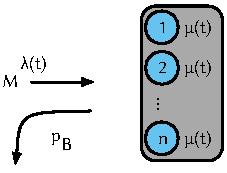
\includegraphics{cloud/virtualized_network_functions/model/figures/traditional_ggsn}
  \caption{Considered model of a traditional \headershortacr{GGSN}.}
  \label{sec:cloud:virtualized_network_functions:model:traditional_ggsn:model}
\end{figure}

We present an abstract queueing model for the traditional \gls{GGSN} in \reffig{sec:cloud:virtualized_network_functions:model:traditional_ggsn:model}.
New tunnels requests arrive according to a Poisson process with rate \(\lambda(t)\) at the \gls{GGSN}.
This server will support a maximum tunnel capacity of \(c\).
When this capacity is reached, blocking will occur and newly incoming tunnels requests are rejected.
Traditionally, \glspl{GGSN} can be expected to be overdimensioned in such a way that this rarely happens.
If the new tunnel is accepted, it will occupy one of the serving units of the server for the duration \(\mu(t)\) of the tunnel.
As stated earlier, we can not model the tunnel duration to be markovian, resulting in a  \(M/GI/c\) loss system.
In order to give quality of service guarantees the network operator is interested in the system's blocking probability \(\blockingprobability\), which we consider to be a key metric of our model.
Additionally, the previously described diurnal patterns can also be modelled by adjusting the arrival and serving process distributions for each time of day.
This alternatively also allows just to investigate the busy hour and thus the system's peak load.

\subsubsection*{\headershortacr{GGSN} using Network Function Virtualisation}\label{sec:cloud:virtualized_network_functions:model:virtual_ggsn}
Next, we introduce concepts from \gls{NFV}, i.e. the idea to replace middleboxes with commodity hardware as an extended model in \reffig{sec:cloud:virtualized_network_functions:model:virtual_ggsn:model}.
This allows us to realise benefits from cloud computing, as we are now able to scale out, instead of up.
The assumptions of the Markov arrival process \(\lambda(t)\) and the serving time distributions \(\mu(t)\) are carried over.
However, instead of one server processing every tunnel, this model assumes that there are up to \(s_{max}\) virtualised servers \(s_i\).
Each of these is less powerful than the traditional \gls{GGSN}, having a tunnel serving capacity of \(c_i \ll c\) and a total system capacity of \(c_{max} = s_{max} \times i\).

\begin{figure}
  \centering
  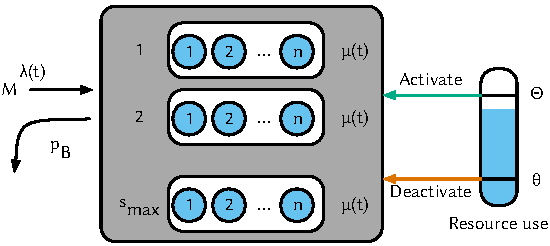
\includegraphics{cloud/virtualized_network_functions/model/figures/virtual_ggsn}
  \caption{Considered model of a virtualised \headershortacr{GGSN}.}
  \label{sec:cloud:virtualized_network_functions:model:virtual_ggsn:model}
\end{figure}

In its initial state, for efficiency, all but a small portion of the server instances are considered to be disabled.
Only, when a certain condition is reached, a new server instance is provisioned.
As a simple example, one instance could be kept in reserve for upcoming requests and an additional would be provisioned as soon as the reserve is used.
Similar rules should apply in the shut-down of servers and form a hysteresis with the boot condition.
For example it would be possible to keep at least one server in reserve but never more than two.

If these conditions are not carefully selected and are in tune with the expected boot time of an instance, additional blocking can occur.
Despite not having reached its maximum capacity, this system would still reject tunnel requests during the provisioning phase when no tunnel slots are available.
This could be remedied by a request queue.
However, this would introduce additional complexity to the system without providing real benefit, as mobile devices or applications will repeat their attempts and would timeout when the request is taking too long.

To place incoming tunnel state on one of the available servers a load balancer is required.
To ensure that the system in run time can scale down to its actual needs, the balancer should place tunnels on servers that are the fullest, keeping the reserve free.
It may even migrate tunnel state from almost empty servers away so that these can be shut down, when the shut-down condition is fulfilled.
Keeping instance close to their capacity should also have no impact on the performance a mobile device associated to a specific tunnel experiences.

\subsection{Measurement Data}\label{sec:cloud:virtualized_network_functions:measurement_data}

In order to evaluate our models introduced in \refsec{sec:cloud:virtualized_network_functions:model}, we use data gathered from a nation-wide mobile operator.
This allows for precise core network evaluations and the creation statistical fits for the observed processes.
In this section we first describe the dataset used for the evaluation and afterwards we derive the random variables required for our models.

\subsubsection*{Dataset Description}\label{sec:cloud:virtualized_network_functions:measurement_data:description}

\label{sec:dataset_description}

All data was collected by the \gls{METAWIN} monitoring system~\cite{Ricciato2006} with measurement probes located at the Gn interface within the core network, enabling broad access to signaling.
For this investigation we employ \gls{GTP} protocol data gathered by \gls{METAWIN}.
This data includes the \gls{RAT} identifier as well as the terminal types of the mobile clients, by use of the \gls{TAC} part of the \gls{IMEI}.
To meet privacy requirements, \gls{METAWIN} anonymizes all captured data.
The application-level payload is removed and all user identifiers are hashed with one-way functions before data storage.
Individual \glspl{UE} in our dataset can be differentiated by the hashed \gls{MS-ID}, but not traced back to the actual user.

The used dataset is a week-long trace from the third week of April 2011.
It consists of \(2.2\) billion aggregated flows for user traffic and \(410\) million \gls{GTP} Tunnel Management transactions.
It was tapped at one of the \glspl{GGSN} of the operator and contains about half of the total traffic volume handled by the operator in this period.

\subsubsection*{Statistical Evaluation}\label{sec:cloud:virtualized_network_functions:measurement_data:evaluation}

Using this dataset, we can obtain the distributions required for the models introduced in \refsec{sec:cloud:virtualized_network_functions:model}.
First, we study the tunnel interarrival time in \reffig{fig:cloud:virtualized_network_functions:measurement_data:evaluation:tunnel_iat}.

\begin{figure}
  \centering
  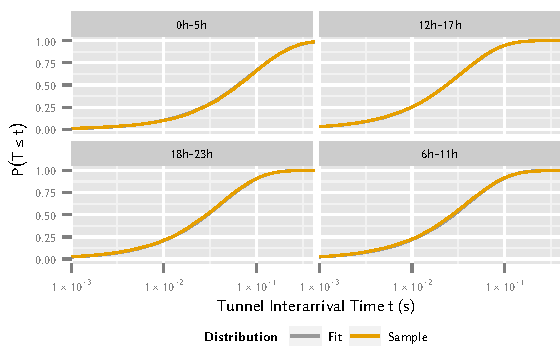
\includegraphics{cloud/virtualized_network_functions/measurement_data/figures/tunnel_iat}
  \caption{Empirical and exponentially fitted CDFs of the tunnel interarrival duration by time of day. CDFs are overlapping as the coefficient of determination is close to \(1\).}
  \label{fig:cloud:virtualized_network_functions:measurement_data:evaluation:tunnel_iat}
\end{figure}

The arrival of new tunnel requests can be used as a measure for the load a \gls{GGSN} experiences, as every incoming tunnel carries several signaling interactions, processing and state with it.
Typically, a device will only hold one tunnel at a time, but this tunnel can be initiated and shut down in rapid succession, causing the aforementioned issues in the radio network.
The arrivals also show a strong diurnal effect, closely resembling patterns present in the actual user traffic:
We observe a decline of arrivals, i.e. longer interarrivals, late in the night and during the early morning hours with a peak rate in the afternoon and early evening.
To represent this time-of-day dependence in the model, the measurement was split into the four time slots displayed in the figure.
Each slot was then fitted with an exponential distribution by way of moment matching.
This results in the cumulative distribution function \(F(x) = 1- e^{-\lambda x}, x \geq 0\) with \(\lambda\) given in \reftab{tab:cloud:virtualized_network_functions:measurement_data:evaluation:iat_fits} for the four time slots.
The fitted functions match the empirical data, with some deviation present at the left tail but overall with a positive correlation coefficient approaching \(1\).

\begin{table}
  \centering
  \caption{Parameters for the exponentially distributed inter-arrival times and corresponding Pearson correlation coefficients}
  \label{tab:cloud:virtualized_network_functions:measurement_data:evaluation:iat_fits}  
  \begin{tabular}{ccc}
  \toprule
  Time of Day & \(\lambda\) & \(R_{arr}\)\\
  \midrule
  0h-5h & $10.67$ & $0.99$\\
  6h-11h & $24.53$ & $0.99$\\
  12h-17h & $29.25$ & $0.99$\\
  18h-23h & $23.49$ & $0.98$\\
   \bottomrule
  \end{tabular}
\end{table}

The second important tunnel property is the duration of the \gls{PDP} Context state accompanying a \gls{GTP} tunnel held at the \gls{GGSN}.
\reffig{fig:cloud:virtualized_network_functions:measurement_data:evaluation:tunnel_duration} shows the tunnel durations split up for the time of day, as there is once again a slight diurnal effect present, albeit with shifted peaks.
Longer tunnels tend to occur at night, shorter tunnels during midday.
Further properties of the tunnel duration, especially the correlation with device types and operating systems, are investigated in detail in~\cite{Metzger2014}.

\begin{figure}
  \centering
  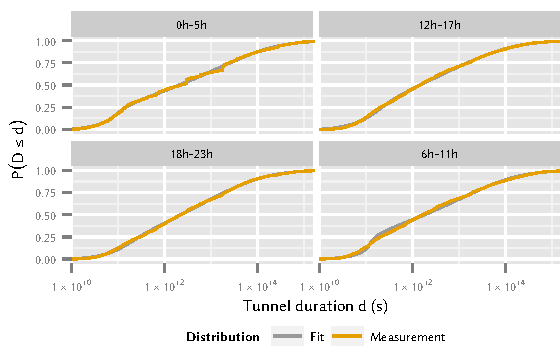
\includegraphics{cloud/virtualized_network_functions/measurement_data/figures/tunnel_duration}
  \caption{Empirical and fitted CDFs of the tunnel duration by time of day with fitted rational functions.}
  \label{fig:cloud:virtualized_network_functions:measurement_data:evaluation:tunnel_duration}
\end{figure}

\begin{table}
  \centering
  \caption{Inverse functions fitted to the empirical duration distribution and correlation coefficients of the fit.}
  \label{tab:cloud:virtualized_network_functions:measurement_data:evaluation:duration_fits}  
  \begin{tabular}{ccc}
  \toprule
  Time of Day & Inverse Fitted Duration Function & \(R_{dur}\)\\
  \midrule
  0h-5h & $0.91 - 60.61y - 3498.78y^3 - \frac{110.70y + 2289.94y^3}{y - 1.00}$ &  $0.99$ \\
  6h-11h & $1 + 117.48y - 368.64y^2 - \frac{1720.13y^4}{y - 1.00}$ & $0.99$ \\
  12h-17h & $0.95 + 69.49y + \frac{81146.10y^3 + 1.08\times10^6y^5}{805 - 802.01y}$ & $0.99$ \\
  18h-23h & $0.91 + 82.05y - \frac{2936.93y^4}{1.94y - 1.95}$ & $0.99$\\
  \bottomrule
  \end{tabular}
\end{table}

Furthermore, the model requires information on the tunnel durations.
However, none of the basic probability distributions, e.g. exponential, gamma, and weibull distributions, fit the tunnel duration well enough.
One of the reasons for this probably being the correlation of the tunnel duration to a large number of factors, including user behavior and network-specific timers and procedures, e.g. tunnels are shut down by the network after specific events, introducing artifacts which make it hard to fit any distribution against.
Instead, we fit rational functions to the empirical \gls{CDF} using the Eureqa \cite{Schmidt2009} software.

This allowes for a much closer fit while still smoothing out some of the artifacts.
\reftab{tab:cloud:virtualized_network_functions:measurement_data:evaluation:duration_fits} displays these functions fitted to the inverse \gls{CDF}, to be directly used for generating random numbers using the inversion method.
Both the \gls{CDF} in \reffig{fig:cloud:virtualized_network_functions:measurement_data:evaluation:tunnel_duration} as well as the Pearson correlation coefficient confirm the goodness of the fitted functions.

\subsection{Inferring State Transitions and Deriving Metrics}\label{sec:network:network_traces:performance_evaluation}
A \gls{UE}’s firmware triggers \gls{RRC} state transitions based on application traffic.
While solutions exist to capture RRC state transitions on specific hardware~\cite{zayas2010} they are not available for all modern smartphone platforms.
Other options to measure the required information include using costly hardware and use specific \glspl{UE}, usually not available to researchers and application developers.
This prevents the developers from evaluating the effect of their applications on the overall health
of the network.
Consequently, they can not take measures to prevent the harmful behaviour of their applications.
However, it is possible to infer the \gls{RRC} state transitions for a given packet trace if the network configuration is known.

First, we describe the setup used to capture network packet traces for arbitrary apps.
Then, we give an algorithm to infer the \gls{RRC} state transitions for a given packet trace.
Based on these state transitions, we can calculate the number of signalling messages generated
by the packet trace. 
Finally, we use the information on when which \gls{RRC} state was entered to calculate the power drain of the \gls{UE}’s radio interface.

\subsubsection*{Measurement Procedure and Setup}\label{sec:network:network_traces:performance_evaluation:measurement}
To investigate the behaviour of the application under study, we capture traffic during a typical use of the application on a \emph{Samsung Galaxy SII} smartphone.
The smartphone runs the Android operating system and is connected to the \gls{3G} network of a major German network operator.
To obtain the network packet traces we use the \texttt{tcpdump} application.
This application requires \emph{root} privileges which are obtained by rooting the device and installing the custom \emph{cyanogenmod} ROM \footnote{\url{http://www.cyanogenmod.org}, Accessed: November, \(21^{st}\) 2015}.
Once \texttt{tcpdump} is installed and running, we start the application under study and capture packet traces while the application is running.
Then, the \emph{android debugging bridge} is used to copy the traces to a workstation.
The traces contain \gls{IP} packets embedded in Linux Cooked Captures.
We require the \gls{IP} packets, thus we extracted the \gls{IP} packets which are used during the analysis to follow.

\subsubsection*{Inferring Network State}\label{sec:network:network_traces:performance_evaluation:inferring_network_state}
In this section we study the influence of the application traffic on \gls{RRC} state transitions and signalling messages.
Since \gls{RRC} state transitions can not be captured using commonly available tools, we introduce an algorithm to infer \gls{RRC} state transitions from \gls{IP} packet traces.
Using this algorithm we analyse the \gls{RRC} state transition frequency and signalling message load for the Two State Model and Three State Model.

Traffic below the network layer can not be measured without specific equipment which interfaces with the proprietary firmware of the \gls{UE} and is often out of reach for developers interested in assessing the impact of their applications on the network.
Based on the Two State and Three State models introduced in \refsec{sec:network:background:umts_rrc}, we process \texttt{tcpdump} captures of the application traffic.
However, it should be noted that this method is not restricted to a specific network model, but can be extended to any other network model as well.
Using these captures, we extract the timestamps when \gls{IP} packets are sent or received.
Furthermore, we require the timer values of the transition from \gls{RRC_DCH} state to \gls{RRC_FACH} state, \gls{TDCH}, and the timer for the transition between \gls{RRC_FACH} and \gls{RRC_idle} states, \gls{TFACH}.
Based on these informations \refalg{alg:network:network_traces:performance_evaluation:inferring_network_state:inference_algorithm} infers the timestamps of state transitions according to the \gls{3GPP} specification \cite{3GPP_RRC_Spec} for the Three State Model.
This algorithm can be simplified to also work for the Two State Model. 
Alternatively, a method to post process the results of the algorithm to obtain results for the Two State Model is given at the end of this section.
The algorithm first computes the inter-arrival times of all packets.
Then, each timestamp is considered.
If the \gls{UE} is currently in \gls{RRC_idle} state, a state transition to \gls{RRC_DCH} occurs at the moment the packet is sent or received.
If the inter-arrival time exceeds the \gls{TDCH} timer the \gls{UE} transitions to \gls{RRC_FACH} \gls{TDCH} seconds after the packet was sent or received.
Similarly, if the inter-arrival time exceeds both the \gls{TDCH} and \gls{TFACH} timers a state transition to \gls{RRC_idle} occurs \gls{TDCH} seconds after the state transition to \gls{RRC_FACH}.

\begin{algorithm}
  \begin{algorithmic}
    \Require{Packet arrival timestamps \emph{ts}\\
    \gls{RRC_DCH} to \gls{RRC_FACH} timer \gls{TDCH}\\
    \gls{RRC_FACH} to \gls{RRC_idle} timer \gls{TFACH}}
    \Ensure{Times of state transition \emph{state\_time}\\
    New states after state transitions \emph{state}}
    \State \texttt{interarrival(i)} $\leftarrow$ \emph{ts}(i+1) - \emph{ts}(i)
    \State \texttt{index} $\leftarrow 0$
    \ForAll{ts(i)}
      \If{\texttt{state(index)} = \gls{RRC_idle}}
        \State \texttt{index} $\leftarrow$ \texttt{index} + 1
        \State \texttt{state(index)} $\leftarrow$ \gls{RRC_DCH}
        \State \texttt{state\_time(index)} $\leftarrow$ ts(i)
      \EndIf
      \If{\texttt{interarrival}(i-1) $> \gls{TDCH}$}
        \State \texttt{index} $\leftarrow$ \texttt{index} + 1
        \State \texttt{state(index)} $\leftarrow$ \gls{RRC_FACH}
        \State \texttt{state\_time(index)} $\leftarrow$ ts(i) $+ \gls{TDCH}$
      \EndIf
      \If{\texttt{interarrival}(i-1) $> \gls{TDCH} + \gls{TFACH}$}
        \State \texttt{index} $\leftarrow$ \texttt{index} + 1
        \State \texttt{state(index)} $\leftarrow$ \gls{RRC_idle}
        \State \texttt{state\_time(index)} $\leftarrow$ ts(i) $+ \gls{TDCH} + \gls{TFACH}$
      \EndIf
    \EndFor
  \end{algorithmic}
  \caption{Inferring \headershortacr{RRC} state transitions based on \headershortacr{IP} timestamps.}
  \label{alg:network:network_traces:performance_evaluation:inferring_network_state:inference_algorithm}
\end{algorithm}

Decreasing power drain of their devices is always a goal of \gls{UE} vendors.
A straightforward way to achieve this, if only the wellbeing of the \gls{UE} is considered, is to transition from \gls{RRC_DCH} state to \gls{RRC_idle} as soon as no additional data is ready for sending.
While this transition is not directly available in the 3GPP specification for the \gls{RRC} protocol \cite{3GPP_RRC_Spec}, a \gls{UE} may reset the connection, effectively transitioning from any state to \gls{RRC_idle}.
This behaviour can be modeled using the Two State Model introduced in \refsec{sec:network:background:umts_rrc}.

State transitions for the Two State Model can be calculated using a similar algorithm.
Alternatively, the behaviour of the Two State Model can be emulated using \refalg{alg:network:network_traces:performance_evaluation:inferring_network_state:inference_algorithm} if \gls{TFACH} is set to \SI{0}{\second} and all state transitions to \gls{RRC_FACH} are removed in a post processing step.

\subsubsection*{Calculating Signalling Frequency and Power Drain}\label{sec:network:network_traces:calculating_metrics}

\begin{table}
\centering
  \caption{Number of signalling messages per \headershortacr{RRC} state transition perceived at the \headershortacr{RNC} \cite{3GPP_RRC_Spec}.}
  \label{tab:network:network_traces:calculating_metrics:signalling_messages}
\begin{tabular}{lccc}
	\toprule
    from/to & \gls{RRC_idle} & \gls{RRC_FACH} & \gls{RRC_DCH}\\
    \midrule
    \gls{RRC_idle} & -- & 28 & 32\\
    \gls{RRC_FACH} & 22 & -- & 6\\
    \gls{RRC_DCH} & 25 & 5 & --\\
    \bottomrule    
	\end{tabular}
\end{table}

In reality, the number of state transitions is not the metric of most importance if network signalling is to be evaluated.
Each state transition results in a number of \gls{RRC} messages between the \gls{UE} and different network components.
For this study we consider the number of messages observed at the \gls{RNC}, which can be found in \cite{3GPP_RRC_Spec} and is summarized in \reftab{tab:network:network_traces:calculating_metrics:signalling_messages}.
It can be seen that transitions from or to the \gls{RRC_idle} state are especially expensive in terms of number of messages sent or received.
This is due to the fact that upon entering or leaving the \gls{RRC_idle} state, authentication has to be performed. 
Note that for the Two State Model only transitions from or to the \gls{RRC_idle} state occur.
This results in the fact that for the same network packet trace the number of signalling messages occurring in the Two State Model is generally higher than in the Three State Model.
To obtain the total number of signalling messages, we weight the number of state transitions with the number of messages sent per state transitions.
Then, we average the number of state transitions over the measurement duration to obtain a metric for the signalling load at the \gls{RNC}, i.e. the \gls{SF}.
The inference algorithm does not differentiate between state changes caused by upstream or downstream traffic.
State changes caused by downstream traffic usually generate some additional signalling messages, as paging is involved.
The inference algorithm can easily be enhanced to support this behaviour.
However, the results discussed in the next section would only change quantitatively.
Furthermore, the algorithm can be adapted to new networking models or other numbers of signalling messages sent per state transition.

\begin{table}
  \centering
  \caption{Power consumption of the \headershortacr{UE} radio interface depending on current \headershortacr{RRC} state \cite{Qian2011a}.}
  \label{tab:network:network_traces:calculating_metrics:power_consumption}  
  \begin{tabular}{lc}
  	\toprule
    \gls{RRC} State & Power Consumption\\
    \midrule
    \gls{RRC_idle} & \SI{0}{\milli\watt}\\
    \gls{RRC_FACH} & \SI{650}{\milli\watt}\\
    \gls{RRC_DCH} & \SI{800}{\milli\watt}\\
    \bottomrule
  \end{tabular}
\end{table}

From a users point of view, the signalling message frequency is of little importantance.
The user is interested in a low power drain as this increases the battery life of the device.
To calculate the battery life, we use the time when state transitions occurred, and the information about the state the transition was to, to calculate the relative amount of time that was spent in each state.
Given the relative time spent in each state, we use \reftab{tab:network:network_traces:calculating_metrics:power_consumption}, taken from \cite{Qian2011a}, to compute the \gls{PD} of the radio interface during the measurement phase.
We focus on the power drain of the radio interface, as it is possible to measure the aggregated power drain using out of the box instrumentation techniques provided by the hardware vendor.
\section{Crowdsourcing Platforms}\label{sec:cloud:crowdsourcing}

\newcommand{\campaignIAT}{\ensuremath{t_c}\xspace}
\newcommand{\campaignSize}{\ensuremath{\Theta}\xspace}
\newcommand{\taskDuration}{\ensuremath{B}\xspace}
\newcommand{\meanTaskLength}{\ensuremath{E[B]}\xspace}
\newcommand{\numberOfWorkers}{\ensuremath{c}\xspace}

\newcommand{\workerUtilization}{\ensuremath{\rho}\xspace}
\newcommand{\campaignDuration}{\ensuremath{\delta}\xspace}
\newcommand{\preTaskProcessingDelay}{\ensuremath{E[D]}\xspace}

\cite{Schwartz2015}

\subsection{Models of \headershortacr{GGSN} Implementations}\label{sec:cloud:virtualized_network_functions:model}

In this section we provide a model for a traditional \gls{GGSN} and discuss a model for a virtual \gls{GGSN} using \gls{NFV}.
In \gls{NFV} \cite{Nfv2013} static network middleboxes are replaced by commodity hardware.
The tasks solved by the original middleboxes are then solved by dedicated software.

\subsubsection*{Traditional GGSN}\label{sec:cloud:virtualized_network_functions:model:traditional_ggsn}
First, we give a model for a \emph{traditional} \gls{GGSN}, i.e. a static network component.
While we consider the \gls{GGSN} to be one fixed entity, it can in reality consist of multiple servers.
However, due to the fact that the \gls{GGSN} is purchased from a vendor as a middlebox, idle servers can be neither deactivated nor reused for other purposes.

\begin{figure}
  \centering
  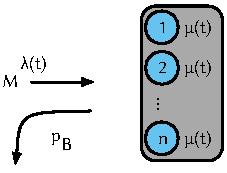
\includegraphics{cloud/virtualized_network_functions/model/figures/traditional_ggsn}
  \caption{Considered model of a traditional \headershortacr{GGSN}.}
  \label{sec:cloud:virtualized_network_functions:model:traditional_ggsn:model}
\end{figure}

We present an abstract queueing model for the traditional \gls{GGSN} in \reffig{sec:cloud:virtualized_network_functions:model:traditional_ggsn:model}.
New tunnels requests arrive according to a Poisson process with rate \(\lambda(t)\) at the \gls{GGSN}.
This server will support a maximum tunnel capacity of \(c\).
When this capacity is reached, blocking will occur and newly incoming tunnels requests are rejected.
Traditionally, \glspl{GGSN} can be expected to be overdimensioned in such a way that this rarely happens.
If the new tunnel is accepted, it will occupy one of the serving units of the server for the duration \(\mu(t)\) of the tunnel.
As stated earlier, we can not model the tunnel duration to be markovian, resulting in a  \(M/GI/c\) loss system.
In order to give quality of service guarantees the network operator is interested in the system's blocking probability \(\blockingprobability\), which we consider to be a key metric of our model.
Additionally, the previously described diurnal patterns can also be modelled by adjusting the arrival and serving process distributions for each time of day.
This alternatively also allows just to investigate the busy hour and thus the system's peak load.

\subsubsection*{\headershortacr{GGSN} using Network Function Virtualisation}\label{sec:cloud:virtualized_network_functions:model:virtual_ggsn}
Next, we introduce concepts from \gls{NFV}, i.e. the idea to replace middleboxes with commodity hardware as an extended model in \reffig{sec:cloud:virtualized_network_functions:model:virtual_ggsn:model}.
This allows us to realise benefits from cloud computing, as we are now able to scale out, instead of up.
The assumptions of the Markov arrival process \(\lambda(t)\) and the serving time distributions \(\mu(t)\) are carried over.
However, instead of one server processing every tunnel, this model assumes that there are up to \(s_{max}\) virtualised servers \(s_i\).
Each of these is less powerful than the traditional \gls{GGSN}, having a tunnel serving capacity of \(c_i \ll c\) and a total system capacity of \(c_{max} = s_{max} \times i\).

\begin{figure}
  \centering
  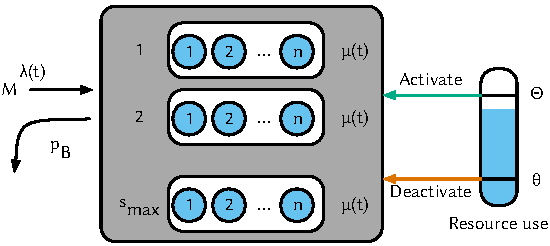
\includegraphics{cloud/virtualized_network_functions/model/figures/virtual_ggsn}
  \caption{Considered model of a virtualised \headershortacr{GGSN}.}
  \label{sec:cloud:virtualized_network_functions:model:virtual_ggsn:model}
\end{figure}

In its initial state, for efficiency, all but a small portion of the server instances are considered to be disabled.
Only, when a certain condition is reached, a new server instance is provisioned.
As a simple example, one instance could be kept in reserve for upcoming requests and an additional would be provisioned as soon as the reserve is used.
Similar rules should apply in the shut-down of servers and form a hysteresis with the boot condition.
For example it would be possible to keep at least one server in reserve but never more than two.

If these conditions are not carefully selected and are in tune with the expected boot time of an instance, additional blocking can occur.
Despite not having reached its maximum capacity, this system would still reject tunnel requests during the provisioning phase when no tunnel slots are available.
This could be remedied by a request queue.
However, this would introduce additional complexity to the system without providing real benefit, as mobile devices or applications will repeat their attempts and would timeout when the request is taking too long.

To place incoming tunnel state on one of the available servers a load balancer is required.
To ensure that the system in run time can scale down to its actual needs, the balancer should place tunnels on servers that are the fullest, keeping the reserve free.
It may even migrate tunnel state from almost empty servers away so that these can be shut down, when the shut-down condition is fulfilled.
Keeping instance close to their capacity should also have no impact on the performance a mobile device associated to a specific tunnel experiences.

\subsection{Measurements}\label{sec:cloud:crowdsourcing:measurements}
In this section we analyse a large dataset from a commercial crowdsourcing platform to derive to derive realistic model parameters and compare the model based on these results with the analytic approximation.

\subsubsection*{Deriving Realistic Model Parameters}
Our analysis is based on a large dataset from the commercial micro-tasking platform Microworkers.com.
The dataset contains information about more then 160.000 campaigns submitted to the platform between May 2009 and Jan 2015, including the number of task per campaign was well as the time of the submission of the campaign.  

\paragraph*{Interarrival Times:} First, we study the inter-arrival times of the campaigns.
During the observation period, the platform faced some downtime due to software update or changes of the technical infrastructure.
During this time, no campaigns could be submitted resulting in relatively large campaign inter-arrival times.
In our model we only consider the regular operation of the platform, therefore we removed all inter-arrival times larger then \SI{97.5}{\percent} quantile of all observed values, which affects about \SI{2.5}{\percent} of all values.

\begin{figure}
  \centering
  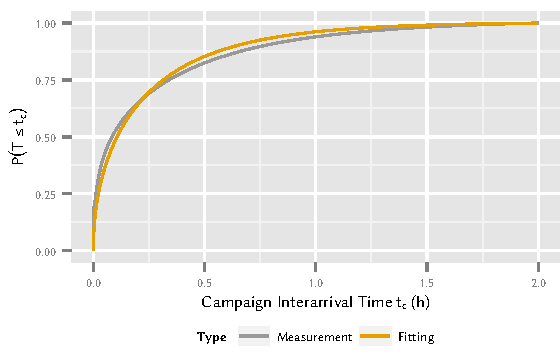
\includegraphics{cloud/crowdsourcing/measurements/figures/campaign_interarrival}
  \caption{Observed campaign inter-arrival times \(t_c\) and corresponding fit.}
  \label{fig:cloud:crowdsourcing:measurements:parameters:campaign_interarrival}
\end{figure}

Considering the remaining data, we observe a mean campaign inter-arrival time of \SI{0.241}{\hour} with a standard deviation \SI{0.346}{\hour}.
\reffig{fig:cloud:crowdsourcing:measurements:parameters:campaign_interarrival} shows the \gls{CDF} of considered inter-arrival times, as well as the fitted distribution.
For the fitting we considered several possible distributions but found the Gamma-distribution 

\[
P(t_c=t) \sim \Gamma(\alpha,\beta,t_c) = \frac{\beta^\alpha}{\Gamma(\alpha)} x^{\alpha-1} e^{-{\beta}t_c}
\]

defined by shape \(\alpha\) and rate \(\beta\) to be the most suitable.
Using \texttt{fitdistrplus} for the R language we derive the distribution parameters by moment fitting and result in the estimated parameters \(\alpha=0.484\) and \(\beta=2.009\).

\paragraph*{Campaign Sizes:}Next, we consider the campaign sizes, respectively the number of tasks per campaign.
The smallest possible campaign sizes on Microworkers is \(30\) tasks, however our dataset contained a few internal test campaigns with a small size.

These test campaigns, as well as outliers larger than the \SI{97.5}{\percent} quantile of the campaign size have been removed from the considered dataset.
In total \SI{3.7}{\percent} of the original dataset were filtered by these conditions, the remaining data resulted in a mean campaign size of \(97.01\) tasks and a standard deviation of \(103.41\).
The CDF of the campaign sizes is depicted in \reffig{fig:cloud:crowdsourcing:measurements:parameters:campaign_sizes}, together with the corresponding fitted distribution.

\begin{figure}
  \centering
  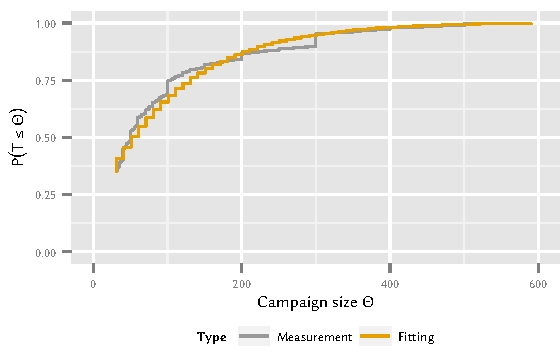
\includegraphics{cloud/crowdsourcing/measurements/figures/campaign_sizes}
  \caption{Observed campaign sizes \campaignSize and corresponding fit.}
  \label{fig:cloud:crowdsourcing:measurements:parameters:campaign_sizes}
\end{figure}

Due to the platform restrictions mentioned above, the campaign sizes start with a minimum value of \(30\) tasks.
We observer that a very high share, i.e. \SI{35}{\percent}, of campaigns has only this minimum size.
Further, campaign sizes which are a multiple of ten or a multiple of \(100\) are quite frequent.
This is caused by the fact that most task on Microworkers.com are repetitive and the employers choose the required number of repetitions and thus are more likely to round the number of repetitions to the nearest multiple of ten or \(100\).

In order to obtain an suitable analytic distribution for the empiric values, we divided the observed values and use the following piecewise defined distribution.
\begin{equation*}
P(S=s) \sim
\begin{cases}
  0 & \text{if } s < s_{\min}\\
  p_{s_{\min}} & \text{if } s=s_{\min} \\
  GEOM(s) \cdot 10 + (s_{\min}+1) & \text{else}
\end{cases}
\end{equation*}
with 
\begin{equation*}
GEOM(s) = {(1-p)}^s p
\end{equation*}
The minimum campaign size \(s_{\min}\) is observed with a fixed probability \(p_{s_{\min}}\), while all campaign sizes larger then \(s_{\min}\) follow a shifted and scaled geometric distribution.

Due to the relatively high frequencies of campaign sizes being multiples of \(10\) and \(100\), it is only possible to achieve a good fitting either for the lower or the higher region of the geometric part.
As an overestimation of the campaign size will give us an upper bound of the platform work load, we decided to put a stronger emphasis on correct fitting of the larger campaign sizes.

Using the \texttt{fitdistrplus} package for the R language we estimate the \(p=0.086\) parameter of the geometric distribution using quantile matching for the \SI{90}{percent} quantile.
The values \(s_{\min}=30\) and \(p_{s_{\min}}=0.350\) are obtained from the empirical values.

\paragraph*{Task Duration: }Another relevant model parameter is the processing time of the tasks, i.e., the time a single worker needs to complete one tasks.
Unfortunately, this information cannot be obtained from our dataset, as tracking of the individual workers is not possible.
Therefore, we assume that the processing times follow a negative-exponential distribution, i.e.
\begin{equation*}
P(t_p=t) \sim \mu  e^{-{\mu}t}
\end{equation*}
Even if the exact processing times are not available, each employer has to add an estimation about the time it task to complete a task in the campaign description.
In our dataset, \SI{87.8}{\percent} of all tasks had an estimated completion time between \SIrange{60}{300}{\second}.
Therefore, we consider \(\mu \in \{\frac{1}{6},\frac{1}{5},\hdots,\frac{1}{2},1\}\) for the following evaluations.

\paragraph*{Number of Workers: }Finally, the last model parameter to estimate is the number of users on the crowdsourcing platform. 
At the time of this analysis, Microworkers.com had over 650.000 registered user accounts.
However, this number is not applicable in the proposed model, for multiple reasons.
The proposed model does not consider vacation times, i.e., the workers would have to be available 24/7.
In reality, many crowdsourcing workers only work occasionally on the platforms or only for a few tasks.
Further, employers can limit the access of to their campaigns to specific subset of all workers, which is also not considered in the model.
Moreover, Microworkers also limits the number of tasks a worker can complete in a single campaign.
Taking this into account, the number of workers to be considered in our model has to be much small then the number of workers on the real world platform and consequently we decided to estimate meaningful values based on the model parameters instead of using the given number of workers from the dataset.

\subsubsection*{Comparison of Detailed and Analytical Model}
An important question for the later analysis is whether the analytic model from \refsec{sec:cloud:crowdsourcing:model} can be used as an approximation or if a simulative evaluation is necessary.
To this end we compared the later considered metrics \workerUtilization and \preTaskProcessingDelay for 
\begin{enumerate*}
\item a simulation using the empiric distributions for the task inter-arrival times and campaign sizes,
\item a simulation using the fitted distributions derived earlier in this section, and
\item the analytic model derived in \refsec{sec:cloud:crowdsourcing:model}.
\end{enumerate*}
For the analytical model we used the campaign size distribution derived in this section and \(\lambda=\SI{4.14}{\per\hour}\).
The results of the different models are shown in \reffig{fig:cloud:crowdsourcing:measurements:comparison:distribution}.

\begin{figure*}
	\centering
	\begin{subfigure}{\columnwidth}
		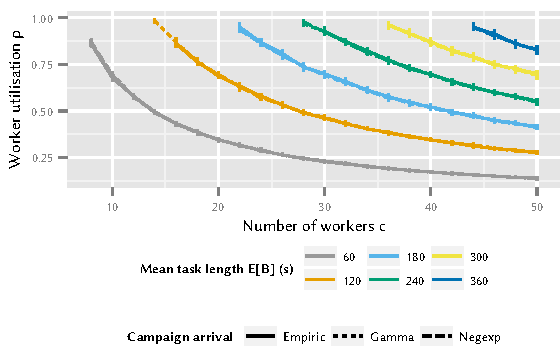
\includegraphics{cloud/crowdsourcing/measurements/figures/distribution_utilization}
		\caption{Worker utilization}
		\label{fig:cloud:crowdsourcing:measurements:comparison:distribution:utilization}
	\end{subfigure}

	\begin{subfigure}{\columnwidth}
		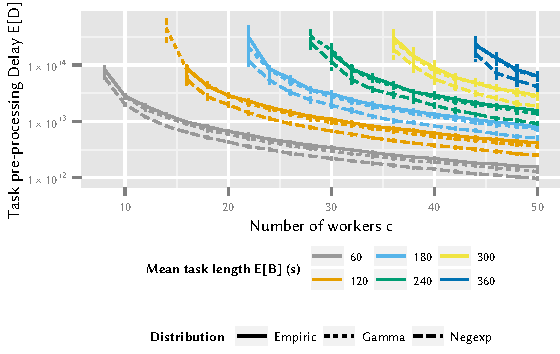
\includegraphics{cloud/crowdsourcing/measurements/figures/distribution_task_delay}
		\caption{Task pre-processing delay}
		\label{fig:cloud:crowdsourcing:measurements:comparison:distribution:task_delay}
	\end{subfigure}
	\caption{Comparison of campaign arrival distributions.}
	\label{fig:cloud:crowdsourcing:measurements:comparison:distribution}
\end{figure*}

The worker utilisation \workerUtilization is depicted in \reffig{fig:cloud:crowdsourcing:measurements:comparison:distribution:utilization}, the task pre-processing delay \preTaskProcessingDelay in \reffig{fig:cloud:crowdsourcing:measurements:comparison:distribution:task_delay}.
In both figures, the x-axis shows the number of workers \(n\).
The line colour indicates the mean task length, ranging from \SIrange{60}{360}{\second}, the line style denotes the underlying model.
We observe that all models result in the same values of \workerUtilization, which is not surprising when considering \(\workerUtilization = \frac{E[t_c] E[\campaignSize]}{c\mu}\) with the mean inter-arrival time \(E[t_c]\).
Here, all parameters are the same for the tree compared models and therefore, no significant differences can be seen.

This is different for the task pre-processing delay \preTaskProcessingDelay. 
Here, large discrepancies can been observed between the model based on the empiric distributions and the analytical model.
This results show that the \(M^{[\campaignSize]}/M/\numberOfWorkers-\infty\) model can also not be used as a worst case estimations, due to the fact that it underestimates \preTaskProcessingDelay.
In contrast to this, the simulation model based on the gamma distribution fit quite accurate the model based on the empirical values.
Therefore, we decide continue our evaluation with the simulation model, based on the gamma distributed inter-arrival times and the piecewise defined distribution for the campaign sizes.

\subsection{Inferring State Transitions and Deriving Metrics}\label{sec:network:network_traces:performance_evaluation}
A \gls{UE}’s firmware triggers \gls{RRC} state transitions based on application traffic.
While solutions exist to capture RRC state transitions on specific hardware~\cite{zayas2010} they are not available for all modern smartphone platforms.
Other options to measure the required information include using costly hardware and use specific \glspl{UE}, usually not available to researchers and application developers.
This prevents the developers from evaluating the effect of their applications on the overall health
of the network.
Consequently, they can not take measures to prevent the harmful behaviour of their applications.
However, it is possible to infer the \gls{RRC} state transitions for a given packet trace if the network configuration is known.

First, we describe the setup used to capture network packet traces for arbitrary apps.
Then, we give an algorithm to infer the \gls{RRC} state transitions for a given packet trace.
Based on these state transitions, we can calculate the number of signalling messages generated
by the packet trace. 
Finally, we use the information on when which \gls{RRC} state was entered to calculate the power drain of the \gls{UE}’s radio interface.

\subsubsection*{Measurement Procedure and Setup}\label{sec:network:network_traces:performance_evaluation:measurement}
To investigate the behaviour of the application under study, we capture traffic during a typical use of the application on a \emph{Samsung Galaxy SII} smartphone.
The smartphone runs the Android operating system and is connected to the \gls{3G} network of a major German network operator.
To obtain the network packet traces we use the \texttt{tcpdump} application.
This application requires \emph{root} privileges which are obtained by rooting the device and installing the custom \emph{cyanogenmod} ROM \footnote{\url{http://www.cyanogenmod.org}, Accessed: November, \(21^{st}\) 2015}.
Once \texttt{tcpdump} is installed and running, we start the application under study and capture packet traces while the application is running.
Then, the \emph{android debugging bridge} is used to copy the traces to a workstation.
The traces contain \gls{IP} packets embedded in Linux Cooked Captures.
We require the \gls{IP} packets, thus we extracted the \gls{IP} packets which are used during the analysis to follow.

\subsubsection*{Inferring Network State}\label{sec:network:network_traces:performance_evaluation:inferring_network_state}
In this section we study the influence of the application traffic on \gls{RRC} state transitions and signalling messages.
Since \gls{RRC} state transitions can not be captured using commonly available tools, we introduce an algorithm to infer \gls{RRC} state transitions from \gls{IP} packet traces.
Using this algorithm we analyse the \gls{RRC} state transition frequency and signalling message load for the Two State Model and Three State Model.

Traffic below the network layer can not be measured without specific equipment which interfaces with the proprietary firmware of the \gls{UE} and is often out of reach for developers interested in assessing the impact of their applications on the network.
Based on the Two State and Three State models introduced in \refsec{sec:network:background:umts_rrc}, we process \texttt{tcpdump} captures of the application traffic.
However, it should be noted that this method is not restricted to a specific network model, but can be extended to any other network model as well.
Using these captures, we extract the timestamps when \gls{IP} packets are sent or received.
Furthermore, we require the timer values of the transition from \gls{RRC_DCH} state to \gls{RRC_FACH} state, \gls{TDCH}, and the timer for the transition between \gls{RRC_FACH} and \gls{RRC_idle} states, \gls{TFACH}.
Based on these informations \refalg{alg:network:network_traces:performance_evaluation:inferring_network_state:inference_algorithm} infers the timestamps of state transitions according to the \gls{3GPP} specification \cite{3GPP_RRC_Spec} for the Three State Model.
This algorithm can be simplified to also work for the Two State Model. 
Alternatively, a method to post process the results of the algorithm to obtain results for the Two State Model is given at the end of this section.
The algorithm first computes the inter-arrival times of all packets.
Then, each timestamp is considered.
If the \gls{UE} is currently in \gls{RRC_idle} state, a state transition to \gls{RRC_DCH} occurs at the moment the packet is sent or received.
If the inter-arrival time exceeds the \gls{TDCH} timer the \gls{UE} transitions to \gls{RRC_FACH} \gls{TDCH} seconds after the packet was sent or received.
Similarly, if the inter-arrival time exceeds both the \gls{TDCH} and \gls{TFACH} timers a state transition to \gls{RRC_idle} occurs \gls{TDCH} seconds after the state transition to \gls{RRC_FACH}.

\begin{algorithm}
  \begin{algorithmic}
    \Require{Packet arrival timestamps \emph{ts}\\
    \gls{RRC_DCH} to \gls{RRC_FACH} timer \gls{TDCH}\\
    \gls{RRC_FACH} to \gls{RRC_idle} timer \gls{TFACH}}
    \Ensure{Times of state transition \emph{state\_time}\\
    New states after state transitions \emph{state}}
    \State \texttt{interarrival(i)} $\leftarrow$ \emph{ts}(i+1) - \emph{ts}(i)
    \State \texttt{index} $\leftarrow 0$
    \ForAll{ts(i)}
      \If{\texttt{state(index)} = \gls{RRC_idle}}
        \State \texttt{index} $\leftarrow$ \texttt{index} + 1
        \State \texttt{state(index)} $\leftarrow$ \gls{RRC_DCH}
        \State \texttt{state\_time(index)} $\leftarrow$ ts(i)
      \EndIf
      \If{\texttt{interarrival}(i-1) $> \gls{TDCH}$}
        \State \texttt{index} $\leftarrow$ \texttt{index} + 1
        \State \texttt{state(index)} $\leftarrow$ \gls{RRC_FACH}
        \State \texttt{state\_time(index)} $\leftarrow$ ts(i) $+ \gls{TDCH}$
      \EndIf
      \If{\texttt{interarrival}(i-1) $> \gls{TDCH} + \gls{TFACH}$}
        \State \texttt{index} $\leftarrow$ \texttt{index} + 1
        \State \texttt{state(index)} $\leftarrow$ \gls{RRC_idle}
        \State \texttt{state\_time(index)} $\leftarrow$ ts(i) $+ \gls{TDCH} + \gls{TFACH}$
      \EndIf
    \EndFor
  \end{algorithmic}
  \caption{Inferring \headershortacr{RRC} state transitions based on \headershortacr{IP} timestamps.}
  \label{alg:network:network_traces:performance_evaluation:inferring_network_state:inference_algorithm}
\end{algorithm}

Decreasing power drain of their devices is always a goal of \gls{UE} vendors.
A straightforward way to achieve this, if only the wellbeing of the \gls{UE} is considered, is to transition from \gls{RRC_DCH} state to \gls{RRC_idle} as soon as no additional data is ready for sending.
While this transition is not directly available in the 3GPP specification for the \gls{RRC} protocol \cite{3GPP_RRC_Spec}, a \gls{UE} may reset the connection, effectively transitioning from any state to \gls{RRC_idle}.
This behaviour can be modeled using the Two State Model introduced in \refsec{sec:network:background:umts_rrc}.

State transitions for the Two State Model can be calculated using a similar algorithm.
Alternatively, the behaviour of the Two State Model can be emulated using \refalg{alg:network:network_traces:performance_evaluation:inferring_network_state:inference_algorithm} if \gls{TFACH} is set to \SI{0}{\second} and all state transitions to \gls{RRC_FACH} are removed in a post processing step.

\subsubsection*{Calculating Signalling Frequency and Power Drain}\label{sec:network:network_traces:calculating_metrics}

\begin{table}
\centering
  \caption{Number of signalling messages per \headershortacr{RRC} state transition perceived at the \headershortacr{RNC} \cite{3GPP_RRC_Spec}.}
  \label{tab:network:network_traces:calculating_metrics:signalling_messages}
\begin{tabular}{lccc}
	\toprule
    from/to & \gls{RRC_idle} & \gls{RRC_FACH} & \gls{RRC_DCH}\\
    \midrule
    \gls{RRC_idle} & -- & 28 & 32\\
    \gls{RRC_FACH} & 22 & -- & 6\\
    \gls{RRC_DCH} & 25 & 5 & --\\
    \bottomrule    
	\end{tabular}
\end{table}

In reality, the number of state transitions is not the metric of most importance if network signalling is to be evaluated.
Each state transition results in a number of \gls{RRC} messages between the \gls{UE} and different network components.
For this study we consider the number of messages observed at the \gls{RNC}, which can be found in \cite{3GPP_RRC_Spec} and is summarized in \reftab{tab:network:network_traces:calculating_metrics:signalling_messages}.
It can be seen that transitions from or to the \gls{RRC_idle} state are especially expensive in terms of number of messages sent or received.
This is due to the fact that upon entering or leaving the \gls{RRC_idle} state, authentication has to be performed. 
Note that for the Two State Model only transitions from or to the \gls{RRC_idle} state occur.
This results in the fact that for the same network packet trace the number of signalling messages occurring in the Two State Model is generally higher than in the Three State Model.
To obtain the total number of signalling messages, we weight the number of state transitions with the number of messages sent per state transitions.
Then, we average the number of state transitions over the measurement duration to obtain a metric for the signalling load at the \gls{RNC}, i.e. the \gls{SF}.
The inference algorithm does not differentiate between state changes caused by upstream or downstream traffic.
State changes caused by downstream traffic usually generate some additional signalling messages, as paging is involved.
The inference algorithm can easily be enhanced to support this behaviour.
However, the results discussed in the next section would only change quantitatively.
Furthermore, the algorithm can be adapted to new networking models or other numbers of signalling messages sent per state transition.

\begin{table}
  \centering
  \caption{Power consumption of the \headershortacr{UE} radio interface depending on current \headershortacr{RRC} state \cite{Qian2011a}.}
  \label{tab:network:network_traces:calculating_metrics:power_consumption}  
  \begin{tabular}{lc}
  	\toprule
    \gls{RRC} State & Power Consumption\\
    \midrule
    \gls{RRC_idle} & \SI{0}{\milli\watt}\\
    \gls{RRC_FACH} & \SI{650}{\milli\watt}\\
    \gls{RRC_DCH} & \SI{800}{\milli\watt}\\
    \bottomrule
  \end{tabular}
\end{table}

From a users point of view, the signalling message frequency is of little importantance.
The user is interested in a low power drain as this increases the battery life of the device.
To calculate the battery life, we use the time when state transitions occurred, and the information about the state the transition was to, to calculate the relative amount of time that was spent in each state.
Given the relative time spent in each state, we use \reftab{tab:network:network_traces:calculating_metrics:power_consumption}, taken from \cite{Qian2011a}, to compute the \gls{PD} of the radio interface during the measurement phase.
We focus on the power drain of the radio interface, as it is possible to measure the aggregated power drain using out of the box instrumentation techniques provided by the hardware vendor.
\section{Lessons Learned}\label{sec:network:lessons_learned}
In this chapter we studied the impact of smartphone application traffic on mobile communication networks.
We considered three stakeholders interacting in the mobile network.
The \emph{mobile network operator} is interested in preventing so called signalling storms, where network components performance is degraded due to high signalling load caused by applications generating network traffic from users' \glspl{UE}.
The \emph{hardware vendor} is interested in satisfying customers by providing a long battery lifetime for the \gls{UE}, i.e. reducing power drain.
The \emph{application developer} is interested in increasing \gls{QoE} for the applications user.
Each of the stakeholders can influence the mobile network, by manipulating the parameters under its control.
The network operator can manipulate \gls{RRC} timers, increasing the time a smartphone stays connected to the network if no data is sent or received, decreasing the number of connections being established or severed and thus the signalling load in the network. 
The hardware vendor can implement proprietary \gls{RRC} protocol extensions, skipping power intensive connection states in order to reduce power drain.
The application developer can shorten update intervals, in order to provide more up to date events and increase \gls{QoE}.
However, each of the parameters under control of the individual stakeholders influence the \glspl{KPI} of the other stakeholders.

This chapter provides a two-pronged approach to analysing the impact of changes by individual stakeholders on the overall network.

First, we provided an algorithm to derive \gls{RRC} state transitions from traffic measurements of already deployed or prototyped applications.
While proprietary mechanisms exist to directly measure \gls{RRC} state transitions, due to the high price they are usually out of reach for application developers, preventing them from evaluating the impact of their applications on the network.
Based on this algorithm we analyse four popular smartphone applications, and find that while it is possible to find a viable tradeoff between signalling load and power drain for single applications, no such tradeoff exists if multiple applications operating in the network at the same time are considered.
For example, for the considered \emph{Twitter} application, increasing the network timer \TDCH from \SI{10}{\second} to \SI{11}{\second} would result in a decrease of signalling by \SI{40}{\percent}, while only resulting in an increase of power drain of \SI{6}{\percent}.
However, if the \emph{Aupeo} application is running in the same network optimised for the Twitter application, this change results in no reduction of signalling load and an increased power drain of \SI{5}{\percent}. 

Furthermore, we show that network timer optimisation, a practice where network operators manipulate \gls{RRC} timers in order to reduce signalling load, incentivises users to enable proprietary fast dormancy algorithms, resulting in a net increase of signalling load.
For example, if a network operator increases the \TDCH network timer from \SI{4}{\second} to \SI{8}{\second}, in order to reduce the signalling frequency caused by the Angry Birds application by \SI{67}{\percent}, this results in an increased power drain at the user's \gls{UE} of \SI{341}{\percent}.
If the user enables the fast dormancy option of the \gls{UE}, the power drain is decreased by \SI{27}{\percent}, however this increases the signalling frequency above the original value before the reconfiguration of the network operator.
%We also show that while longer \gls{RRC} timers may have an adverse effect on power drain due to the smartphone being longer connected to the network, it results in an increase of Web \gls{QoE}, as this results in web pages being able to be loaded faster if the smartphone is already connected to the network.

Second, we propose an analytical model to derive the \glspl{KPI} from analytical or empirical traffic distributions, in order to evaluate the impact of applications that do not yet exist or classes of applications defined by a common traffic characteristics.
Our results show that different access patterns have a considerable impact on the required resources of the mobile phone and the network.
We identified bursty traffic pattern as particularly resource-efficient with respect to power drain and signalling load.
In contrast, nearly periodic traffic is likely to cause signalling overload due to frequent connection re-establishments, especially when the connection timeout is slightly below the inter-packet time.
This can be observed on the example of a \TDCH timer of \SI{10}{\second}.
Here, the coefficient of variation has no impact on the signalling load for very small inter-packet times \(E[\PacketIAT]<\SI{1e-1}{\second}\) or very large inter-packet times \(E[\PacketIAT]>\SI{1e3}{\second}\).
For example, for a mean inter-arrival time of \(E[\PacketIAT] = 11.5\) seconds, an increase of coefficient of variation from \(0.5\) to \(5.0\) can decrease the signalling load by \SI{53}{\percent}.

Concluding from this chapter, we see that in mobile networks many different players, metrics, and tradeoffs exist.
We highlighted one examples of such a tradeoff, i.e. signalling load vs. power drain and discussed the influence of the current optimisation parameters, the network timers, on another.
However, many additional tradeoffs exist.
For example, the mobile operator has to balance the use of radio resources with the number of generated signalling frequencies.
Furthermore, application providers seek to improve the user experience which usually result in a higher frequency of network polls, creating additional signalling traffic.
The high number of tradeoffs and involved actors in this optimisation problem indicate that the current optimisation technique used by operators is no longer sufficient.

Approaches like \emph{Economic Traffic Management}~\cite{spirou2009} or \emph{Design for Tussle}~\cite{trilogy2008} could be applied to find
an acceptable tradeoff for all parties.
In Economic Traffic Management all participating entities share information in order to enable collaboration.
This collaboration allows for a joint optimisation of the tradeoff.
Design for Tussle aims to resolve tussles at run time, instead instead of design time.
This prevents the case that one actor has full control over the optimisation problem, which would likely result in the actor choosing a tradeoff only in its favour, ignoring all other participants.
One example of an actor providing information for another in order to optimise the total system would be \gls{UE} vendor providing interfaces for application developers to use when sending data.
These interfaces would schedule data to be transmitted in such a way that signalling load and power drain would be reduced, if the application’s requirements allow for it.
Until such interfaces exist, application developers could take the effect of the traffic their applications
produce both on the \gls{UE} and the network into account, for example using the algorithms proposed in this chapter. 